\documentclass[11pt]{article}
\usepackage[T1]{fontenc}
\usepackage[utf8]{inputenc}
\usepackage{lmodern}
\usepackage[margin=1.03in]{geometry}
\usepackage{amsmath,amssymb,amsthm,mathtools,mathrsfs}
\usepackage{enumitem,booktabs,array,longtable,graphicx}
\usepackage{tikz}
\usetikzlibrary{arrows.meta,positioning,calc,decorations.pathreplacing}
\usepackage{microtype}
\usepackage[hidelinks]{hyperref}
\usepackage{bookmark}
\urlstyle{same}
\hypersetup{
  pdftitle={The Deligne-Drinfeld conjecture},
  pdfauthor={OpenAI},
  pdfsubject={The Deligne-Drinfeld conjecture},
  pdfkeywords={Grothendieck-Teichmuller Lie algebra, Deligne-Drinfeld conjecture, Ihara bracket}
}
\newcommand{\Q}{\mathbb Q}
\newcommand{\Z}{\mathbb Z}
\newcommand{\F}{{\mathbb F_2}}
\newcommand{\CC}{\mathbb C}
\newcommand{\Lie}{\operatorname{Lie}}
\newcommand{\grt}{\mathfrak{grt}_1}
\DeclareMathOperator{\ad}{ad}
\DeclareMathOperator{\wt}{wt}
\DeclareMathOperator{\depth}{depth}
\DeclareMathOperator{\gr}{gr}
\newcommand{\id}{\mathrm{id}}
\newtheorem{theorem}{Theorem}[section]
\newtheorem{proposition}[theorem]{Proposition}
\newtheorem{lemma}[theorem]{Lemma}
\newtheorem{corollary}[theorem]{Corollary}
\theoremstyle{definition}
\newtheorem{definition}[theorem]{Definition}
\theoremstyle{remark}
\newtheorem{remark}[theorem]{Remark}
\numberwithin{equation}{section}
\setcounter{tocdepth}{1}
\setlist{topsep=4pt,itemsep=2pt,parsep=0pt}
\setlength{\emergencystretch}{1em}

\title{The Deligne--Drinfeld conjecture}
\author{OpenAI}
\date{September 23, 2026}
\begin{document}
\maketitle
\begin{abstract}
We prove the Deligne--Drinfeld conjecture: the rational Grothendieck--Teichm\"uller Lie algebra is freely generated by one element in every odd weight at least three, with the corresponding isomorphism after weight completion.
\end{abstract}
\tableofcontents
\section{Introduction}\label{sec:introduction}

The Grothendieck--Teichm\"uller Lie algebra records the infinitesimal
symmetries of the associativity and braiding constraints for
parenthesized braids.  Its defining equations are short, but they place
conditions in every weight on a free Lie algebra in two letters.
The Deligne--Drinfeld conjecture predicts that these conditions leave
exactly a free Lie algebra with one generator in each odd weight
starting at three.  We prove this conjecture, including generation of
the entire solution space.

\subsection{The statement}
Let \(L=\Lie_{\Q}\langle x,y\rangle\), graded by the total number of
letters.  We call this degree the \emph{weight}.  For a finite set of
labels, the infinitesimal pure braid Lie algebra \(\mathfrak t_n\)
has generators \(t_{ij}=t_{ji}\), \(i\ne j\), and relations
\begin{equation}\label{eq:braid-relations}
 [t_{ij},t_{k\ell}]=0\quad(i,j,k,\ell\text{ distinct}),\qquad
 [t_{ij},t_{ik}+t_{jk}]=0\quad(i,j,k\text{ distinct}).
\end{equation}
Every generator has weight one.
Let \(W\subset L\) be the graded vector space of polynomials satisfying
\begin{align}
 \psi(x,y)+\psi(y,x)&=0,\label{eq:antisymmetry}\\
 \psi(x,y)+\psi(y,-x-y)+\psi(-x-y,x)&=0.\label{eq:three-term}
\end{align}
\begin{equation}\label{eq:pentagon}
\begin{aligned}
 &\psi(t_{12},t_{23}+t_{24})+\psi(t_{13}+t_{23},t_{34})\\
 &\qquad=
 \psi(t_{23},t_{34})+\psi(t_{12}+t_{13},t_{24}+t_{34})
 +\psi(t_{12},t_{23}).
\end{aligned}
\end{equation}
The last equation is imposed in \(\mathfrak t_4\).
These are the usual defining equations of \(\grt\);
see \cite[Section~6.1]{Willwacher}.  We work first with their polynomial
solution space \(W=\bigoplus_n W_n\), where \(W_n\) is its weight-\(n\)
piece.  The usual completed algebra is \(\widehat W=\prod_n W_n\).

For \(\psi\in L\), define the derivation
\begin{equation}\label{eq:ihara-derivation}
 D_\psi(x)=0,\qquad D_\psi(y)=[y,\psi].
\end{equation}
The Ihara bracket, with the convention used throughout this paper, is
\begin{equation}\label{eq:ihara}
 \{\psi,\phi\}=D_\psi(\phi)-D_\phi(\psi)+[\psi,\phi].
\end{equation}

\begin{theorem}\label{thm:main}
There are homogeneous elements
\(\sigma_{2k+1}\in W_{2k+1}\), one for each \(k\ge1\), for which
\[
 \Lie_{\Q}\langle e_3,e_5,e_7,\ldots\rangle
 \longrightarrow (W,\{\, ,\,\}),\qquad
 e_{2k+1}\longmapsto\sigma_{2k+1},
\]
is an isomorphism of graded Lie algebras.
In particular, \(W\) is closed under the bracket
\eqref{eq:ihara}.  The induced map on completions by weight is a
continuous graded isomorphism.
\end{theorem}

The generators in Theorem~\ref{thm:main} are not canonical.
The assertion combines two requirements: there are no additional Lie
relations among them, and they span every solution of
\eqref{eq:antisymmetry}--\eqref{eq:pentagon}.

\subsection{Context and the main estimate}
The arithmetic study of the fundamental group of the projective line
minus three points provides a central setting for these symmetry
questions; Deligne developed its motivic and tangential-basepoint
framework in \cite[Introduction and Section~15]{Deligne}.
Drinfeld's associators express compatibility between reassociation and
braiding, and their symmetries led to the
Grothendieck--Teichm\"uller group and its Lie algebra
\cite{Drinfeld}.  The equations above are the corresponding
infinitesimal compatibility conditions.

The conjecture has three parts: existence of the proposed odd-weight
elements, freeness of the Lie algebra they generate, and exhaustion of
the equation space.  Drinfeld's Proposition~6.3 credits Ihara with the
odd-weight existence result and gives an associator proof.
Brown's work on mixed Tate motives over \(\mathbb Z\) proves the
faithfulness of the motivic action on the fundamental group of the
three-punctured line \cite{Brown}.  The graded Lie algebra of the
prounipotent motivic Galois group is free on generators corresponding to weights
\(3,5,7,\ldots\); its inclusion in the associator symmetry algebra
therefore supplies a free Lie subalgebra of \(W\)
\cite[Section~1.4.2]{BrownDepth}.
Willwacher subsequently proved freeness for any homogeneous family of
solutions, one in each odd weight \(2k+1\ge3\), whose corresponding
element has nonzero coefficient of
\(x^{2k}y\) \cite[Theorem~1.2]{WillwacherFree}.
This coefficient lies in the \emph{depth-one} component, consisting of
words with exactly one occurrence of \(y\).

Freeness leaves open whether there are additional solutions of the
defining equations; see \cite[Section~9]{Willwacher}.
Naef and Willwacher's computations of the linearized
Kashiwara--Vergne algebra, together with the known inclusions,
establish the required equality through weight~29
\cite[Theorem~5 and Corollary~7]{NaefWillwacher}.
Our main estimate is the all-weight upper bound
\[
 \dim_{\Q}W_n\leq
 \dim_{\Q}\Lie_{\Q}\langle e_3,e_5,e_7,\ldots\rangle_n,
 \qquad \wt(e_j)=j,
\]
proved in Corollary~\ref{cor:dimension-bound} for the full rational
equation space.  The known free subalgebra gives the reverse inequality.
The proof here also obtains that lower bound internally:
Sections~\ref{sec:category}--\ref{sec:induction} construct a rational
subspace of solutions closed under the Ihara bracket, supply its
odd-weight depth-one values, and choose integral generators attaining
the bound.  These choices connect the rational construction to the
characteristic-two argument.

The completed assertion has a graph-theoretic consequence.  Over
\(\Q\), Willwacher's isomorphism
\cite[Theorem~1.1]{Willwacher} identifies the zeroth cohomology of
Kontsevich's graph complex with \(\widehat W\).  Thus
\[
 H^0(\mathrm{GC}_2)\cong
 \widehat{\Lie_{\Q}\langle e_3,e_5,e_7,\ldots\rangle}.
\]
The graph complex and its completion are taken in the conventions of
that source.  The superscript zero is a cohomological degree, whereas
the generator indices specify weights; no other cohomological degree
is computed here.

\subsection{Proof strategy}

The main step is a degeneration of the pentagon in characteristic two.
Inside the free associative algebra, put
\[
 A=x^2,\qquad C=[x,y],\qquad B=y,
\]
and filter by the number of occurrences of \(B\).
The pentagon for a leading part becomes a relation in the enveloping
algebra of the level-two cyclotomic hyperplane arrangement
\cite[Section~1.4]{Enriquez}, modulo terms of lower count.
The comparison uses a common ordering procedure: corrections
raise the count in the braid algebra and lower it in the arrangement
algebra.  Keeping only the common count-preserving terms transfers the
relation without any independence assumption on the target algebra.

Integral deletion operators on words then detect the leading part
after setting \(A=0\).  Their analytic antecedents are the
total-differential formulas for iterated integrals and hyperlogarithms
of Goncharov \cite[Theorem~2.1]{Goncharov} and
Panzer \cite[Lemma~3.3.30]{Panzer}.
The operators used here specialize the integral
algebraic differential operators of Hirose and Sato
\cite[Section~2]{HiroseSato}; their use with cyclotomic braid algebras
and ratios of sums and differences follows Hirose's construction
\cite[Sections~4.3 and~6]{Hirose}.  Here the arrangement relations are proved over the
integers before reduction, and the characteristic-two comparison is
proved directly.  A shift symmetry
\(B\mapsto B+s(C)\), followed by a Vandermonde argument, confines the
image to the ordinary free Lie algebra on
\[
 \ad_C^kB,\qquad k\ge1.
\]
These letters have exactly the weights predicted by the conjecture.
The ordering comparison and the integral deletion test provide
separate tools for extracting information from filtered braid
relations.

To attain the bound within the proof, we construct rational solutions with a nonzero
coefficient of \(x^{n-1}y\) in every odd weight \(n\ge3\).
Following Drinfeld's associator proof
\cite[Proposition~6.3]{Drinfeld}, we compare regularized braid holonomy
with the rule obtained by conjugating paths and negating the chord
generators.  We implement
this comparison in the parenthesized-chord formalism of Bar-Natan
\cite[Sections~2--3]{BarNatan}, with the required operations and
limits proved explicitly.  The logarithm of the comparison,
evaluated on a reassociation arrow, has the required nonzero
coefficient.  This uses the nonvanishing of a convergent integral,
and requires no arithmetic independence assertion about its values.

Finally, we work with saturated lattices over \(\Z_{(2)}\).
The characteristic-two bound applies to reductions of rational
solutions.  Independent Hall words in previously chosen generators,
together with a new depth-one value in odd weight, attain the bound
at each step.
Equality forces the next integral generator to occupy the required
leading filtration piece.  This proves generation and freeness
simultaneously.

\subsection{Organization and conventions}
Section~\ref{sec:algebra} establishes the integral algebra and a
special-derivation identity.  Sections~\ref{sec:degeneration}--\ref{sec:image}
prove the dimension bound.  Sections~\ref{sec:category}
and~\ref{sec:holonomy} construct the odd-weight values.
Section~\ref{sec:induction} completes the induction.

All Lie algebras in characteristic two are \emph{ordinary} Lie
algebras, with \([u,u]=0\).  Their enveloping algebras are ordinary
associative enveloping algebras.  We never identify all primitive
elements in characteristic two with ordinary Lie elements.
All completions are by weight, and all infinite constructions are
interpreted first in each finite weight quotient.

\section{Integral Lie algebras and the special identity}
\label{sec:algebra}

Throughout, a Lie algebra is an ordinary Lie algebra: its bracket is
alternating, including in characteristic two.  Put
\(R=\Z_{(2)}=\{a/b\in\Q:b\text{ is odd}\}\), with residue field
\(\F=R/2R\).  We will pass from the rational solution space to an
embedded reduction of the same dimension.  For this passage we need
torsion-free integral targets for the defining equations, together with
an additional identity proved over \(\Q\) before reduction.

\begin{lemma}\label{lem:low-weights}
The solution spaces \(W_1\) and \(W_2\) are zero.
\end{lemma}
\begin{proof}
For \(\psi(x,y)=\alpha x+\beta y\), the left side minus the right side of
the pentagon is \(-\alpha t_{12}-\beta t_{34}\).  The degree-one braid
generators are linearly independent, so \(\alpha=\beta=0\).
The degree-two free Lie algebra is spanned by \([x,y]\), and the
three-term expression for this polynomial is \(3[x,y]\).  Thus it too
has no nonzero rational solution.
\end{proof}

\begin{samepage}
\begin{lemma}[Ordinary Lie lattices]\label{lem:lie-lattice}
Let \(X\) be a finite alphabet, and let \(K(X)\) be the \(R\)-span of
all bracket monomials in the free associative algebra
\(R\langle X\rangle\).  It is the free ordinary Lie algebra over \(R\).
Each multihomogeneous piece is finite free, and its rationalization and
reduction are, respectively,
\[
 K(X)\otimes_R\Q=\Lie_{\Q}\langle X\rangle,
 \qquad
 K(X)/2K(X)=\Lie_{\F}\langle X\rangle
       \ \subset\ \F\langle X\rangle.
\]
In particular, this reduction is injective in associative words, and
free ordinary Lie dimensions in every multidegree agree over \(\Q\)
and \(\F\).  The same statements hold for an alphabet with positive
integer weights and finitely many letters in each bounded weight.
\end{lemma}
\end{samepage}
\begin{proof}
We recall the integral free-Lie and PBW facts being used.  The
Hall--Lyndon construction gives a basis of the free Lie algebra over
\(\Z\): iterated use of alternation and Jacobi expresses bracket
monomials in the standard Lyndon brackets, and the associative
expansion of each such bracket has its Lyndon word as leading word,
with coefficient one.  Distinct leading words give independence over
every coefficient ring.  Thus base change to \(R\) identifies the
abstract free Lie algebra with precisely the displayed bracket span.
PBW applies to this free \(R\)-module; in particular its universal
enveloping algebra is \(R\langle X\rangle\).  These are the usual
integral versions of the free-Lie basis and PBW theorems
\cite[Theorems~0.2, 0.5, 4.9 and~5.1]{Reutenauer};
the integral Lyndon and PBW bases are also recalled in
\cite[Section~2]{MelanconReutenauer}.

The same Lyndon brackets form bases after base change to $\Q$ and
$\F$, with unchanged multidegrees.  This proves the asserted
injectivity and equality of dimensions.  For a weighted alphabet,
restriction to any bounded weight leaves finitely many letters,
so the same basis argument applies.
\end{proof}

In particular, ordinary Lie membership is a condition stronger than
being primitive in a characteristic-two enveloping algebra.  For
example, \(x^2\) is primitive in \(\F\langle x\rangle\), whereas the
ordinary Lie algebra generated by \(x\) is just \(\F x\).  We will
always retain ordinary Lie membership when using associative words.

For a coefficient ring \(k\in\{R,\Q,\F\}\), write
\(\mathfrak t_q(k)\) for the infinitesimal braid Lie algebra on
\(q\) strands, with the presentation in \eqref{eq:braid-relations}.

\begin{lemma}[The free fiber]\label{lem:free-fiber}
The map \(\mathfrak t_q(k)\longrightarrow\mathfrak t_{q-1}(k)\)
which forgets the last strand is split, and its kernel is the free
ordinary Lie algebra on \(s_i=t_{iq}\), \(1\leq i<q\).  Explicitly,
\begin{equation}\label{eq:free-fiber}
 \mathfrak t_q(k)
  =\Lie_k\langle s_1,\ldots,s_{q-1}\rangle
        \rtimes\mathfrak t_{q-1}(k),
\end{equation}
where a base generator \(t_{ij}\) acts by the derivation
\begin{equation}\label{eq:free-fiber-action}
 D_{ij}(s_i)=[s_i,s_j],\qquad
 D_{ij}(s_j)=[s_j,s_i],\qquad
 D_{ij}(s_h)=0\quad(h\notin\{i,j\}).
\end{equation}
Multiplication gives an isomorphism of \(k\)-modules
\begin{equation}\label{eq:enveloping-fiber}
 k\langle s_1,\ldots,s_{q-1}\rangle
       \otimes_k U(\mathfrak t_{q-1}(k))
       \xrightarrow{\ \sim\ }U(\mathfrak t_q(k)).
\end{equation}
Thus recursive products of free associative fiber words are a basis.
Over \(R\), the Lie algebra and its enveloping algebra are torsion
free, and this normal form commutes with rationalization and reduction.
\end{lemma}
\begin{proof}
Any prescription on free generators extends uniquely to a derivation.
Derivations \(D_{ij}\) and \(D_{hk}\) with disjoint supports commute.
For three distinct indices \(i,j,h\), put
\(S_{ijh}=s_i+s_j+s_h\).  On the free subalgebra on these three letters,
\[
 D_{ij}+D_{ih}+D_{jh}:z\longmapsto[z,S_{ijh}].
\]
Moreover \(D_{ij}(S_{ijh})=0\), so \(D_{ij}\) commutes with this sum.
On every other free generator all these derivations vanish.  It
follows that \([D_{ij},D_{ih}+D_{jh}]=0\) on the whole free Lie
algebra.  Hence \eqref{eq:free-fiber-action} defines an action of the
presented base algebra.

Form its semidirect product with the free Lie algebra on the \(s_i\).
The braid relations involving the last strand say precisely
\[
 [t_{ij},s_h]=0\ (h\notin\{i,j\}),\quad
 [t_{ij},s_i+s_j]=0,\quad
 [s_i,t_{ij}+s_j]=[s_j,t_{ij}+s_i]=0.
\]
They hold by \eqref{eq:free-fiber-action}.  Conversely, these relations
in the presented braid algebra give exactly that action.  The maps
between the presented algebra and the semidirect product, taking each
generator to its namesake, are consequently inverse.  This proves
both the presentation and the assertion about the actual kernel.

Inductively the base is a free \(k\)-module.  Choose Lie bases for
fiber and base, and place the entire fiber basis before the base
basis.  PBW identifies their ordered products with a basis of the
enveloping algebra.  Since the enveloping algebra of a free Lie
algebra is the free associative algebra, this is exactly
\eqref{eq:enveloping-fiber}.  Induction, starting with one strand,
gives the asserted word basis.  Lemma~\ref{lem:lie-lattice} and the
same basis over \(R\), \(\Q\), and \(\F\) give the last assertions.
\end{proof}

We next deduce an additional identity from the defining equations.
The first conclusion below is Drinfeld's special identity
\cite[Proposition~5.7]{Drinfeld}.  We give a direct proof that also
establishes the stated linearization.  We use the convention
\(\ad_a(z)=[a,z]\).

\begin{lemma}[The special identity]\label{lem:special}
Let \(\psi\in W_n\), where \(n>2\).  In the free Lie algebra on
\(a,b\), with \(c=-a-b\), one has
\begin{equation}\label{eq:special}
 [a,\psi(b,a)]+[c,\psi(b,c)]=0.
\end{equation}
In addition, for an extra free letter \(T\),
\begin{equation}\label{eq:special-linearization}
 \partial_2\psi(a,-a)T=0,
\end{equation}
where \(\partial_2\) means the coefficient of a central parameter
\(t\) in \(\psi(a,-a+tT)\).
\end{lemma}
\begin{proof}
All calculations in this proof take place over \(\Q\).  We first
rewrite the pentagon in a free kernel, then linearize at \(a+b+c=0\).
Equality of mixed derivatives will force the possible linearization
coefficient to vanish.

\emph{The free-fiber identity.}
Forget strand \(2\) in \(\mathfrak t_4(\Q)\), and put
\[
 a=t_{12},\qquad b=t_{23},\qquad c=t_{24},\qquad
 u=t_{13},\qquad v=t_{34}.
\]
By Lemma~\ref{lem:free-fiber}, the kernel is the actual free Lie
algebra on \(a,b,c\).  Define
\begin{align*}
 F_a&=\psi(u+b,v)-\psi(u,v),\\
 F_b&=\psi(u+a,v+c)-\psi(u,v),\\
 F_c&=\psi(u,v+b)-\psi(u,v).
\end{align*}
Forgetting the fiber sends each displayed difference to zero, so
\(F_a,F_b,F_c\) are elements of this free kernel.  They are
homogeneous of degree \(n\).

Each of the three expressions before subtracting \(\psi(u,v)\)
commutes with its corresponding letter.  For example,
\([a,u+b]=[a,v]=0\) and
\([b,u+a]=[b,v+c]=0\); the third case is the same braid relation at
\(c\).  The base action fixes \(S=a+b+c\).  Summing the resulting
commutators therefore gives
\[
 [a,F_a]+[b,F_b]+[c,F_c]=0.
\]
Set \(\Delta_a=F_b-F_a\) and \(\Delta_c=F_b-F_c\).  We obtain the
identity in the free fiber
\begin{equation}\label{eq:special-fiber}
 [S,F_b]=[a,\Delta_a]+[c,\Delta_c].
\end{equation}

The pentagon gives
\(\Delta_a=\psi(a,b+c)-\psi(a,b)-\psi(b,v)\).
The element \(v+b+c\) is central in the subalgebra on \(v,b,c\).
A Lie polynomial of degree greater than one is unchanged when a
central element is added to an argument: every term in the difference
contains that element in a bracket.  Thus \(\psi(b,v)=\psi(b,-b-c)\).
Exchanging strands \(1\) and \(4\) in the same calculation and using
antisymmetry gives the second formula below:
\begin{align}
 \Delta_a&=\psi(a,b+c)-\psi(a,b)-\psi(b,-b-c),
       \label{eq:special-delta-a}\\
 \Delta_c&=-\psi(c,a+b)+\psi(c,b)+\psi(b,-b-a).
       \label{eq:special-delta-c}
\end{align}
Both differences vanish when \(S=0\): the two remaining terms cancel
by antisymmetry and \(\psi(z,-z)=0\) in degree greater than one.

The ideal generated by \(S\) is stable under the base action, so the
quotient fiber is \(\Lie_{\Q}\langle a,b\rangle\), with
\(c=-a-b\).  In this quotient the actions of \(u,v\) are
\(\ad_c,\ad_a\), respectively.  For example,
\[
 [u,a]=[a,b]=[c,a],\quad [u,b]=[b,a]=[c,b],\quad [u,c]=0,
\]
and
\([v,a]=0\), \([v,b]=[b,c]=[a,b]\),
\([v,c]=[c,b]=[a,c]\).  It follows that \(\psi(u,v)\) acts on
the quotient fiber by \(\ad_{\psi(c,a)}\).  Since the expression
defining \(F_b+\psi(u,v)\) commutes with \(b\), we have
\[
 [b,F_b+\psi(c,a)]=0
\]
in this free Lie quotient.

The centralizer of \(b\) in the ordinary free Lie algebra on \(a,b\)
is \(\Q b\).  To see this directly, embed it in associative words.
For a homogeneous polynomial \(P=\sum_w p_w w\) commuting with
\(b\), comparison in \(bP=Pb\) gives
\(p_{av}=0\) and
\(p_{b^j av}=p_{b^{j-1}avb}\) for every word \(v\) and \(j>0\).
Iterating shows that every word containing \(a\) has coefficient
zero.  Hence \(P\) is a polynomial in \(b\).  Setting \(a=0\) now shows that a
Lie element of this form belongs to the one-dimensional ordinary
Lie algebra on \(b\).  The homogeneous element at hand has degree
\(n>1\), and is therefore zero.  We have proved an equality of
quotient fiber elements, not just of their induced derivations:
\begin{equation}\label{eq:special-fb}
 F_b\big|_{S=0}=-\psi(c,a).
\end{equation}

\emph{The first variation at \(S=0\).}
We have determined the quotient value of \(F_b\).  We now differentiate
\eqref{eq:special-fiber} transversely to this quotient and compare the
result with the derivative of the expression in \eqref{eq:special}.
All subsequent derivatives mean coefficient
extraction after adjoining free direction letters and commuting
scalar parameters.  Thus
\[
 \partial_1\psi(p,q)T=[t]\psi(p+tT,q),\qquad
 \partial_2\psi(p,q)T=[t]\psi(p,q+tT).
\]
The degree-\(n\) Lie polynomials on \(a,T\) containing exactly one
\(T\) and \(n-1\) copies of \(a\) form the one-dimensional space
spanned by \(\ad_a^{n-1}T\): in a nonzero bracket monomial, each
branch not containing \(T\) must be a single \(a\).  Consequently
there is a scalar \(k\in\Q\), depending only on \(\psi\), such that
\begin{equation}\label{eq:special-k}
 \partial_2\psi(a,-a)T=k\ad_a^{n-1}T.
\end{equation}
Differentiating the identity \(\psi(a,-a)=0\) while varying both
arguments gives
\begin{equation}\label{eq:special-diagonal}
 \partial_1\psi(a,-a)T=\partial_2\psi(a,-a)T.
\end{equation}

Take \(c=S-a-b\), keep \(a,b\) fixed, and extract the coefficient
linear in \(S=tT\).  In these same coordinates the two differences
are
\begin{align*}
 \Delta_a&=\psi(a,S-a)-\psi(a,b)-\psi(b,a-S),\\
 \Delta_c&=-\psi(S-a-b,a+b)+\psi(S-a-b,b)+\psi(b,-b-a).
\end{align*}
Writing \(c=-a-b\) after differentiation, their derivatives at zero
are exactly
\begin{align*}
 d_S\Delta_a(T)
   &=k\ad_a^{n-1}T+\partial_2\psi(b,a)T,\\
 d_S\Delta_c(T)
   &=-\partial_1\psi(c,-c)T+\partial_1\psi(c,b)T\\
   &=-k\ad_c^{n-1}T-\partial_2\psi(b,c)T.
\end{align*}
The last equality uses \eqref{eq:special-diagonal} and
antisymmetry.  In differentiating \eqref{eq:special-fiber}, the left
side becomes \([T,F_b|_{S=0}]\): its other product-rule term has
outside letter \(S=0\).  On the right the outside \(a\) is fixed,
and the derivative of the outside \(c\) contributes
\([T,\Delta_c|_{S=0}]=0\).  Thus no outside-letter term remains,
and \eqref{eq:special-fb} gives
\begin{equation}\label{eq:special-transverse}
 \begin{split}
 -[T,\psi(c,a)]={}&k(\ad_a^n-\ad_c^n)T\\
 &+[a,\partial_2\psi(b,a)T]
       -[c,\partial_2\psi(b,c)T].
 \end{split}
\end{equation}

Now define
\(G(a,b)=[a,\psi(b,a)]+[c,\psi(b,c)]\), where \(c=-a-b\).
Hold \(b\) fixed and vary \(a\) in direction \(T\), so that \(c\)
varies in direction \(-T\).  The full product rule is
\begin{align*}
 d_aG(T)={}&[T,\psi(b,a)-\psi(b,c)]\\
           &+[a,\partial_2\psi(b,a)T]
              -[c,\partial_2\psi(b,c)T].
\end{align*}
The three-term identity and antisymmetry give
\(\psi(b,a)-\psi(b,c)=\psi(c,a)\).  Comparing with
\eqref{eq:special-transverse}, we conclude that
\begin{equation}\label{eq:special-dg}
 d_aG(T)=-k(\ad_a^n-\ad_c^n)T.
\end{equation}

\emph{Vanishing of the scalar obstruction.}
Equation~\eqref{eq:special-dg} expresses the derivative of \(G\) in
terms of the single scalar \(k\).  To show that this scalar is zero,
introduce two independent constant directions \(U,V\).  The
coefficients of their two commuting scalar parameters in \(G\)
are unchanged when the differentiations are interchanged.  After
forming these mixed derivatives, specialize
\[
 a=a_0,\qquad b=-a_0,\qquad c=0,\qquad U=a_0,\qquad V=T,
\]
where \(a_0,T\) are free letters.  The derivative of \(\ad_c^n\)
vanishes there, since every summand contains \(n-1>0\) copies of
\(\ad_c\).  The two derivatives of the other term are
\begin{align*}
 d_U(\ad_a^nV)\big|&=n\ad_{a_0}^nT,\\
 d_V(\ad_a^nU)\big|
   &=\sum_{j=0}^{n-1}
       \ad_{a_0}^{j}\ad_T\ad_{a_0}^{n-1-j}a_0
     =-\ad_{a_0}^{n}T.
\end{align*}
Only \(j=n-1\) survives in the second sum.  Equality of the mixed
derivatives in \eqref{eq:special-dg} implies
\[
 (n+1)k\ad_{a_0}^{n}T=0.
\]
The word \(a_0^nT\) has coefficient one in
\(\ad_{a_0}^{n}T\).  Since the calculation is over \(\Q\), it
follows that \(k=0\).  This proves
\eqref{eq:special-linearization}.

Equation~\eqref{eq:special-dg} now says that every directional
derivative of \(G\) in \(a\) vanishes.  Equivalently, setting the
direction equal to \(a\) multiplies its component with \(j\)
occurrences of \(a\) by \(j\).  In characteristic zero every such
component with \(j>0\) is zero.  Thus \(G\) is independent of
\(a\), and evaluation at \(a=0,c=-b\) gives \(G=0\).  This is
\eqref{eq:special}.
\end{proof}

\begin{proposition}[Saturated reduction]\label{prop:saturated-reduction}
Let
\[
 K_n=\Lie_R\langle x,y\rangle_n,
 \qquad L_n=W_n\cap K_n.
\]
Then \(L_n\) is a saturated finite free \(R\)-submodule of \(K_n\),
and its reduction embeds in \(K_n/2K_n\).  Writing its image as
\(\overline L_n\), one has
\begin{equation}\label{eq:saturated-dimension}
 \dim_{\F}\overline L_n=\dim_{\Q}W_n.
\end{equation}
More generally, for any rational subspace \(V_n\subset W_n\), the
lattice \(M_n=V_n\cap K_n\) has an embedded reduction
\(\overline M_n\subset\overline L_n\) of dimension
\(\dim_{\Q}V_n\).

Every element of \(\overline L_n\) satisfies the reductions of the
three defining identities.  If \(n>2\), it also satisfies
\eqref{eq:special} and \eqref{eq:special-linearization} after
reduction, together with all formal coefficient consequences of
these identities.  In particular, putting \(z=x+y\),
\begin{equation}\label{eq:special-mod-two}
 [x,\overline\psi(x,y)+\overline\psi(z,y)]
       +[y,\overline\psi(z,y)]=0
 \qquad(\overline\psi\in\overline L_n).
\end{equation}
\end{proposition}
\begin{proof}
An intersection of a rational subspace with a finite free
\(R\)-module is saturated: if \(v\in K_n\) and \(2v\in L_n\),
then \(v\in W_n\), hence \(v\in L_n\).  Thus
\(L_n\cap2K_n=2L_n\), which gives the asserted injection after
reduction.  It is a finite free module because \(R\) is a principal
ideal domain.  Clearing denominators in a rational basis of
\(W_n\) shows that \(\Q L_n=W_n\), so its rank and its reduction
dimension are \(\dim_{\Q}W_n\).  Exactly the same argument applies
to \(M_n\); embedding both reductions in \(K_n/2K_n\) proves their
stated inclusion.

For a representative \(\psi\in L_n\), each defining identity is
an expression with coefficients in \(R\).  Its target is either a
free Lie lattice or the braid Lie algebra over \(R\).  These targets
embed in their rationalizations by Lemmas~\ref{lem:lie-lattice} and
\ref{lem:free-fiber}.  An expression which vanishes over \(\Q\)
therefore already vanishes over \(R\), and can be reduced modulo
two.  The identical argument applies to the special identity and
its linearization, which were established over \(\Q\) in
Lemma~\ref{lem:special}.  Adjoining free letters and commuting
parameters preserves the word bases; extracting a parameter
coefficient involves no division and commutes with reduction.
This justifies the assertion about formal coefficient consequences.

Finally, reduce \eqref{eq:special}, take \(a=x,b=y,c=x+y\), and
use the reduced antisymmetry to replace \(\overline\psi(y,x)\)
and \(\overline\psi(y,x+y)\) by
\(\overline\psi(x,y)\) and \(\overline\psi(x+y,y)\).
Expanding the outside bracket with \(x+y\) gives
\eqref{eq:special-mod-two}.
\end{proof}

In the characteristic-two arguments that follow, the permitted
polynomials are these reductions of rational solutions.  No
identification of \(\overline L_n\) with the full solution space of
equations written over \(\F\) is asserted or needed.  In particular,
the characteristic-zero mixed-derivative argument proving
\((n+1)k=0\) has already been completed before reduction.

\section{A filtered degeneration of the pentagon}
\label{sec:degeneration}

We now work over $\F$.  The elements to which we apply the
argument are the reductions $\bar\psi\in\overline L_n$ of
Proposition~\ref{prop:saturated-reduction}, with $n>2$.  In particular,
they are ordinary Lie polynomials and satisfy the reduced pentagon.
We first introduce a filtration in which a leading part of that pentagon
can be tested in a different Lie algebra.

\begin{samepage}
\begin{lemma}\label{lem:abc-free}
The assignments
\[
 A\longmapsto x^2,\qquad C\longmapsto[x,y],\qquad B\longmapsto y
\]
define an injective homomorphism
$\F\langle A,C,B\rangle\longrightarrow\F\langle x,y\rangle$.
Its restriction embeds the ordinary free Lie algebra
$\Lie_{\F}\langle A,C,B\rangle$ in the latter associative algebra.
Every homogeneous element of $\Lie_{\F}\langle x,y\rangle$ of weight
greater than one belongs to this embedded Lie algebra.
\end{lemma}
\end{samepage}

\begin{proof}
Order words of each fixed length lexicographically with $x>y$.
The leading words of $x^2,[x,y],y$ are respectively $xx,xy,y$, each with
coefficient one.  These form a prefix code: none is a proper initial
segment of another.  Thus their concatenations have unique decodings,
so distinct words in $A,C,B$ have distinct leading words.  Split a
putative relation by its total $x,y$ length and take the largest
leading word in each part; its coefficient proves associative
injectivity.  Ordinary free Lie algebras embed in their free associative
enveloping algebras, so the Lie assertion follows as well.

We use the ordinary free-Lie elimination construction
\cite[Theorem~0.6]{Reutenauer}, whose needed instance can be seen directly.
Set $e_j=\ad_x^j y$ for $j\geq0$.  The Lie subalgebra generated by the
$e_j$ is stable under $\ad_x$, because $\ad_x(e_j)=e_{j+1}$ and
$\ad_x$ is a derivation.  Its sum with the line $\F x$ is therefore a
Lie algebra containing $x,y$, hence the whole free Lie algebra.  The
subalgebra is thus an ideal with one-dimensional quotient spanned by
the class of $x$.  Every homogeneous Lie polynomial of weight greater
than one consequently lies in this subalgebra.  It is itself free on
the $e_j$: their leading words $x^j y$ form a prefix code, which proves
injectivity of the corresponding free associative algebra and hence
of its ordinary free Lie algebra.

In characteristic two, the associative identity
$\ad_x^2(P)=[x^2,P]$ gives
\begin{equation}\label{eq:elimination-abc}
 e_{2i}=\ad_A^i B,\qquad e_{2i+1}=\ad_A^i C\qquad(i\geq0).
\end{equation}
Both expressions belong to the ordinary Lie algebra on the three
abstract letters $A,C,B$, which proves the final assertion.
\end{proof}

The statement does not assert that $x^2$ is an ordinary Lie polynomial
in $x,y$.  Rather, it embeds an ordinary Lie algebra on three new
letters into an associative algebra; the original Lie polynomials of
weight greater than one happen to lie in its image.

Give $A,C$ weight two and $B$ weight one, and let $F^r$ be the span of
ordinary Lie monomials containing at least $r$ occurrences of $B$.
The multigrading of the free Lie algebra makes this a decreasing
filtration.  Through Lemma~\ref{lem:abc-free}, we regard
$\overline L_n$ as a subspace of
$\Lie_{\F}\langle A,C,B\rangle$ and give it the induced filtration
$F^r\overline L_n=\overline L_n\cap F^r$; write
$\operatorname{gr}^r_F\overline L_n=
F^r\overline L_n/F^{r+1}\overline L_n$.
Write $\Psi(A,C,B)$ for the unique polynomial representing
$\bar\psi$ under Lemma~\ref{lem:abc-free}.  If $\Psi\in F^r$, let
$\chi(A,C,B)$ be its component containing exactly $r$ letters $B$.
Whenever $\chi\ne0$, there is an integer $m\geq0$ such that
\begin{equation}\label{eq:leading-count-weight}
 n=2m+r,
\end{equation}
and every associative word of $\chi$ has $m$ letters from $\{A,C\}$
and total length $m+r$.  The case $m=0$ is zero: an ordinary Lie
polynomial in $B$ alone has only its degree-one component, whereas
$n>2$.  Thus a nonzero leading part always has $m>0$, and in particular
$n>r$.  We shall later study the ordinary Lie polynomial
$f=\chi(0,C,B)$.  This section establishes the relation satisfied by
$\chi$ before that projection.

We need two algebras with the same named symbols.  The source is the
ordinary enveloping algebra of the infinitesimal braid Lie algebra
on strands $0,1,\ldots,d$, over $\F$.  In it put
\begin{equation}\label{eq:source-symbols}
\begin{gathered}
 X_i=t_{0i},\qquad u_{ij}=t_{ij},\qquad
 a_i=X_i^2,\\
 v_{ij}=[X_i,u_{ij}]=[X_j,u_{ij}]=[X_i,X_j].
\end{gathered}
\end{equation}
The equalities defining $v_{ij}$ follow from the three-strand braid
relations and characteristic two.  Here the $a_i$ are associative
squares.

For the target, let $\mathcal A_d$ be the arrangement in $\Q^d$ with
hyperplanes
\[
 \begin{gathered}
 z_i=0\quad(1\leq i\leq d),\\
 z_i-z_j=0,\qquad z_i+z_j=0\quad(1\leq i<j\leq d).
 \end{gathered}
\]
Let $\mathfrak h_{\Z,d}$ be the ordinary Lie algebra over $\Z$ with
one generator $t_H$ for each $H\in\mathcal A_d$ and relations
\begin{equation}\label{eq:flat-relations}
 \left[t_H,\sum_{K\supset T}t_K\right]=0
 \qquad(H\supset T),
\end{equation}
where $T$ ranges over the codimension-two intersections of the
arrangement and the sum ranges over its hyperplanes containing $T$.
This is the level-two cyclotomic infinitesimal braid arrangement
\cite[Section~1.4]{Enriquez}.  We use the integral incidence
presentation \eqref{eq:flat-relations}, not a characteristic-zero
freeness assertion.
All intersections in this definition are taken over $\Q$.
Set $\mathfrak h_d=\mathfrak h_{\Z,d}\otimes\F$, and write
\[
 \begin{gathered}
 a_i=t_{\{z_i=0\}},\qquad
 u_{ij}^s=t_{\{z_i-sz_j=0\}}\quad(s\in\{+1,-1\}),\\
 u_{ij}=u_{ij}^{+1},\quad v_{ij}=u_{ij}^{+1}+u_{ij}^{-1}.
 \end{gathered}
\]
Thus plus and minus hyperplanes remain distinct generators even after
scalar reduction.  For $d=3$ abbreviate these Lie algebras to
$\mathfrak h_\Z$ and $\mathfrak h$.  Each target symbol $a_i,v_{ij},u_{ij}$
has enveloping degree one.

The \emph{count} of a word in either named alphabet is its number of
$u$ symbols; $a,v$ symbols have count zero.  Count is attached to an
expression in the generators, not asserted to be a grading of either
quotient algebra.  We can now state the relation to be transferred.

\begin{proposition}\label{prop:leading-pentagon}
Let $\bar\psi\in\overline L_n$, $n>2$, and suppose its expression
$\Psi(A,C,B)$ lies in $F^r$.  Let $\chi$ be its component of count $r$,
and write $n=2m+r$, with $m>0$.  In $U(\mathfrak h)$ let
$\mathcal U_{\ell,<r}$ be the span of all products of exactly $\ell$
symbols from $\{a_i,v_{ij},u_{ij}\}$ that contain fewer than $r$
symbols $u$.  Then
\begin{equation}\label{eq:leading-pentagon}
\begin{split}
 0\equiv{}&\chi(a_1,v_{12}+v_{13},u_{12}+u_{13})
       +\chi(a_2+v_{12},v_{23},u_{23})\\
 &+\chi(a_1+a_2+v_{12},v_{13}+v_{23},u_{13}+u_{23})\\
 &+\chi(a_1,v_{12},u_{12})\pmod{\mathcal U_{m+r,<r}}.
\end{split}
\end{equation}
For $r=0$ the indicated lower-count subspace is zero.
\end{proposition}

The lower-count remainder belongs to the stated linear subspace of
words of fixed target length $m+r$.  In the next section, scalar deletion
tests on words of length $m+r$ containing $r$ zeros will annihilate
this subspace.
To prove the proposition, we compare
ordering calculations in the two alphabets; no homomorphism between
the two algebras is used.  In the source, terms omitted from the leading
pentagon have higher count; in the target, the permitted remainder has
lower count.  We will show that source ordering never lowers count and
target ordering never raises it, with identical count-preserving parts.

Add a newest strand $d$.  The old symbols
are called base symbols; the new symbols are called fiber symbols.
In the source write
\[
 X=X_d,\qquad H=X^2,\qquad
 U_i=u_{id},\qquad V_i=[X,U_i]\quad(i<d),
\]
and in the target write
\[
 H=a_d,\qquad U_i^s=u_{id}^s,\qquad
 U_i=U_i^{+1},\qquad V_i=U_i^{+1}+U_i^{-1}.
\]
In this notation count includes the $U$ symbols, while $H,V$ have
count zero.  The following exact formulas will justify the two
opposite count inequalities.

\begin{lemma}\label{lem:action-tables}
All commutators of a base symbol with a fiber symbol are given by the
following formulas.  In both algebras use the abbreviations
\[
 R_i=[H,U_i],\qquad Q_i=[H+V_i,U_i],\qquad
 W_{ij}=[V_i,U_j]+[U_i,V_j].
\]
In the source the exact formulas are
\begin{align}
 [a_i,H]&=[H,V_i]+[R_i,U_i],\notag\\
 [a_i,U_i]&=Q_i,& [a_i,U_k]&=0\quad(k\ne i),\notag\\
 [a_i,V_i]&=[H,V_i]+[[V_i,U_i],U_i],\notag\\
 [a_i,V_k]&=[Q_i,U_k]\quad(k\ne i),
 \label{eq:source-a-actions}
\end{align}
\begin{align}
 [u_{ij},H]&=0,\notag\\
 [u_{ij},U_i]&=[u_{ij},U_j]=[U_i,U_j],\notag\\
 [u_{ij},V_i]&=[u_{ij},V_j]=W_{ij},\notag\\
 [u_{ij},U_k]&=[u_{ij},V_k]=0\quad(k\notin\{i,j\}),
 \label{eq:source-u-actions}
\end{align}
and
\begin{align}
 [v_{ij},H]&=[H,[U_i,U_j]],\notag\\
 [v_{ij},U_i]&=[U_i,V_j],&
 [v_{ij},U_j]&=[U_j,V_i],\notag\\
 [v_{ij},V_i]&=[V_i,V_j]+[W_{ij},U_i]+[U_i,R_j],\notag\\
 [v_{ij},V_j]&=[V_i,V_j]+[W_{ij},U_j]+[U_j,R_i],\notag\\
 [v_{ij},U_k]&=0\quad(k\notin\{i,j\}),\notag\\
 [v_{ij},V_k]&=[W_{ij},U_k]\quad(k\notin\{i,j\}).
 \label{eq:source-v-actions}
\end{align}
In the target the exact formulas are
\begin{align}
 [a_i,H]&=[H,V_i],& [a_i,U_i]&=Q_i,\notag\\
 [a_i,V_i]&=[H,V_i],&
 [a_i,U_k]&=[a_i,V_k]=0\quad(k\ne i),
 \label{eq:target-a-actions}
\end{align}
\begin{align}
 [u_{ij},H]&=0,\notag\\
 [u_{ij},U_i]&=[u_{ij},U_j]=[U_i,U_j],\notag\\
 [u_{ij},V_i]&=[u_{ij},V_j]=W_{ij}+[V_i,V_j],\notag\\
 [u_{ij},U_k]&=[u_{ij},V_k]=0\quad(k\notin\{i,j\}),
 \label{eq:target-u-actions}
\end{align}
and
\begin{align}
 [v_{ij},H]&=0,\notag\\
 [v_{ij},U_i]&=[U_i,V_j],&
 [v_{ij},U_j]&=[U_j,V_i],\notag\\
 [v_{ij},V_i]&=[v_{ij},V_j]=[V_i,V_j],\notag\\
 [v_{ij},U_k]&=[v_{ij},V_k]=0\quad(k\notin\{i,j\}).
 \label{eq:target-v-actions}
\end{align}
Every source output has at least the count of its input pair; every
target output has at most that count.  The parts preserving count
are identical in the two lists and have symbolic length two.
\end{lemma}

\begin{proof}
For the source, the braid relations give the following derivations
on its free fiber on $X,U_1,\ldots,U_{d-1}$:
\[
 \begin{aligned}
 \delta_i=\ad_{X_i}:&\quad
 X\longmapsto V_i,\quad U_i\longmapsto V_i,\quad
 U_k\longmapsto0\ (k\ne i),\\
 \epsilon_{ij}=\ad_{u_{ij}}:&\quad
 X\longmapsto0,\quad U_i,U_j\longmapsto[U_i,U_j],\quad
 U_k\longmapsto0\ (k\notin\{i,j\}).
 \end{aligned}
\]
The derivation rule and $[X,V_i]=[X^2,U_i]=R_i$ imply
\[
 \delta_iH=R_i,\qquad \delta_iV_i=Q_i,\qquad
 \delta_iV_k=[V_i,U_k]\quad(k\ne i).
\]
Since $\ad_{a_i}=\delta_i^2$, applying $\delta_i$ again gives
\eqref{eq:source-a-actions}.  For its incident $V_i$ entry, in
particular, $R_i+Q_i=[V_i,U_i]$ gives
\[
 \delta_iQ_i=[R_i+Q_i,U_i]+[H+V_i,V_i]
 =[ [V_i,U_i],U_i]+[H,V_i].
\]
Applying $\epsilon_{ij}$ to $H,V_k$ gives
\eqref{eq:source-u-actions}, since
$[X,[U_i,U_j]]=W_{ij}$.

Next $\ad_{v_{ij}}=[\delta_i,\epsilon_{ij}]$ sends $X$ to $W_{ij}$,
sends $U_i$ to $[U_i,V_j]$, sends $U_j$ to $[U_j,V_i]$, and kills the
other $U_k$.  Its action on $H$ is
$[X,W_{ij}]=[H,[U_i,U_j]]$.  Its remaining actions follow uniformly
from
\[
 [v_{ij},V_k]=[W_{ij},U_k]+[X,[v_{ij},U_k]],
\]
which proves \eqref{eq:source-v-actions}, including the nonincident
entries.

For the target, the flat where $z_i=z_d=0$ lies in exactly the four
hyperplanes with generators $a_i,H,U_i^{+1},U_i^{-1}$.  Its relations give
\[
 [a_i,H]=[H,V_i],\qquad
 [a_i,U_i^t]=[H+V_i,U_i^t]\quad(t\in\{+1,-1\}).
\]
Summing the second formula over $t$ proves the $V_i$ entry of
\eqref{eq:target-a-actions}.  The signed triple flat containing
$u_{ij}^s,U_i^t,U_j^{st}$ gives
\[
 [u_{ij}^s,U_i^t]=[U_j^{st},U_i^t],\qquad
 [u_{ij}^s,U_j^t]=[U_i^{st},U_j^t].
\]
Substitute $U_k^{-1}=U_k+V_k$.  For example,
\[
 \begin{aligned}
 [u_{ij},V_i]
 &=[U_j,U_i]+[U_j+V_j,U_i+V_i]\\
 &=W_{ij}+[V_i,V_j].
 \end{aligned}
\]
Summing also over $s$ gives
$[v_{ij},U_i]=[U_i,V_j]$ and
$[v_{ij},V_i]=[V_i,V_j]$; exchanging $i,j$ gives the other incident
entries.  Every remaining pair in the claimed zero entries meets
in a flat contained in just those two hyperplanes, so its generators
commute.  This proves all target formulas.

The count assertions can now be read term by term.  In the source,
the terms beyond the common quadratic terms add two $U$'s.  In the
target, the only extra term is $[V_i,V_j]$ in
\eqref{eq:target-u-actions}, whose count is zero instead of one.
This also proves agreement of the parts preserving count.
\end{proof}

For clarity, their common incident actions are the short table
\begin{equation}\label{eq:common-actions}
\begin{array}{c|ccc}
 &H&U_i&V_i\\ \hline
 a_i &[H,V_i]&[H+V_i,U_i]&[H,V_i]\\
 u_{ij}&0&[U_i,U_j]&[U_i,V_j]+[V_i,U_j]\\
 v_{ij}&0&[U_i,V_j]&[V_i,V_j]
\end{array}
\end{equation}
with the exchanged-index versions supplied by the full formulas
above and zero common actions at nonincident indices.

We next specify exactly how to use the tables.  At a fixed newest
strand, scan a word from left to right for its first adjacent pair
$bf$ consisting of a base symbol followed by a fiber symbol.  Replace
it by
\begin{equation}\label{eq:ordering-swap}
 bf=fb+[b,f],
\end{equation}
using the appropriate exact formula of
Lemma~\ref{lem:action-tables} and expanding brackets into associative
words.  Fix the order of those expansions once and for all.
On each resulting branch the lexicographic pair
\[
 \bigl(\text{number of base symbols},\,
        \text{number of base-before-fiber inversions}\bigr)
\]
strictly decreases.  The swapped branch lowers the second entry;
every commutator branch removes a base symbol and inserts only fiber
symbols, hence lowers the first entry.  This proves termination even
for a source correction that increases symbolic length.  When all
fiber letters precede the base suffix, repeat the procedure on that
suffix with one fewer strand.  The result is an iterated ordered
expression with the newest fiber first.

There are two further facts about this algorithm.  First, in the
source its ordered products are linearly independent.  Indeed,
Lemma~\ref{lem:free-fiber} identifies the ordinary enveloping algebra,
as a vector space, with the tensor product of the free associative
fiber algebras in this order.  In each fiber the subalgebra generated
by $H,V_i,U_i$ is free associative: with $X$ larger than all $U_i$,
these elements have the respective leading words
\[
 XX,\qquad XU_i,\qquad U_i.
\]
They again form a prefix code.  Thus distinct words in each restricted
fiber alphabet are independent, and so are their ordered products
over all fibers.  At the final one-strand stage this says simply
that the powers of $X_1^2$ are independent.

Second, source ordering never lowers count, while target ordering
never raises it.  This remains true through every recursive stage,
since the unchanged surrounding word contributes the same count
and the action formulas have the required inequality term by term.
A source branch that has acquired count greater than $r$ can never
contribute at count $r$; a target branch of count less than $r$ can
never return to count $r$.  Consequently the branches that preserve
count throughout are described in both algebras by exactly the same
algorithm using \eqref{eq:common-actions}.

\begin{proof}[Proof of Proposition~\ref{prop:leading-pentagon}]
Relabel the four braid strands $0,1,2,3$.  Since signs disappear over
$\F$, the reduced pentagon says that the sum of
\[
 \begin{gathered}
 \bar\psi(X_1,u_{12}+u_{13}),\qquad
 \bar\psi(X_2+u_{12},u_{23}),\qquad
 \bar\psi(u_{12},u_{23}),\\
 \bar\psi(X_1+X_2,u_{13}+u_{23}),\qquad
 \bar\psi(X_1,u_{12})
 \end{gathered}
\]
is zero in the source.  Express these five terms using $\Psi$.
Their exact triples of arguments $(A,C,B)$ are, in the same order,
\begin{equation}\label{eq:five-substitutions}
\begin{aligned}
 &(a_1,\ v_{12}+v_{13},\ u_{12}+u_{13}),\\
 &(a_2+v_{12}+u_{12}^2,\ v_{23}+[u_{12},u_{23}],\ u_{23}),\\
 &(u_{12}^2,\ [u_{12},u_{23}],\ u_{23}),\\
 &(a_1+a_2+v_{12},\ v_{13}+v_{23},\ u_{13}+u_{23}),\\
 &(a_1,\ v_{12},\ u_{12}).
\end{aligned}
\end{equation}
In particular,
\[
 (X_2+u_{12})^2=a_2+v_{12}+u_{12}^2,
 \qquad (X_1+X_2)^2=a_1+a_2+v_{12}.
\]
Only the former square has a $u_{12}^2$ summand.

Expand the pentagon as a polynomial in the restricted source symbols
before ordering.  Its part of count exactly $r$ is precisely the
four-term polynomial $P$ on the right of
\eqref{eq:leading-pentagon}.  To verify this, the higher components
of $\Psi$ already have more than $r$ occurrences of $B$, each of
which becomes a single $u$.  Either extra summand $u_{12}^2$ or
$[u_{12},u_{23}]$ in the second triple increases count by two.
The third triple, being entirely in the $u$ alphabet, gives count
$n>r$.  All remaining replacements preserve the original $B$-count.
Thus the full source pentagon has the form $P+E=0$, where every word
of $E$ has count greater than $r$.

The distinction between original weight and symbolic length is
essential here.  Assign source weight two to each $a,v,H,V$ and
weight one to each $u,U$.  A word of length $\ell$ and count $q$ has
original weight
\begin{equation}\label{eq:weight-length-count}
 n=2\ell-q.
\end{equation}
All source action formulas preserve this weight.  Thus a correction
that raises count by two raises length by one, and every ordered
word of weight $n$ and count $r$ has length
$(n+r)/2=m+r$.  In particular $P$ has that length, while the
higher-count expressions are allowed to have greater length.

Apply the deterministic source ordering to $P+E=0$.  Since count
never decreases, $E$ contributes nothing at count $r$.  Independence
of the ordered restricted source products, proved above from the
free fibers, implies that every ordered coefficient of count $r$
in $P$ is zero separately.  This conclusion uses independence
across all the restricted words, so expressions of other lengths
or counts cannot cancel a coefficient under consideration.

Now interpret only the polynomial $P$, of length $m+r$, in the
target.  Apply the same deterministic ordering, discarding a branch
as soon as its count falls below $r$.  Such a branch can never return
to count $r$.  The retained branches use the identical quadratic
formulas that retained count $r$ in the source.  Their ordered
coefficient vector is therefore the zero vector just obtained.
Every target replacement preserves length, so every discarded
branch has length $m+r$ and count less than $r$.  Their sum belongs
to $\mathcal U_{m+r,<r}$, proving \eqref{eq:leading-pentagon}.

Only source independence enters this argument.  In the target the
ordering procedure is a sequence of valid equalities yielding a
spanning expression; no independence or free-fiber assertion for
$\mathfrak h$ is required.
\end{proof}

\section{Deletion operators and injectivity of the leading projection}
\label{sec:deletion}

Our goal is to show that setting $A=0$ loses no leading part
$\chi(A,C,B)$ of a reduced rational solution.  We use deletion
operators to test the four-term relation of
Proposition~\ref{prop:leading-pentagon}.  These tests first show that
a leading part killed by $A=0$ can involve only $A,B$; the special
identity then excludes this remaining kernel.

\subsection{The integral deletion representation}
The operators below specialize the integral algebraic differential
operators of Hirose and Sato \cite[Section~2]{HiroseSato}.
Their logarithmic-form and cyclotomic braid interpretation follows
Hirose's construction \cite[Section~4.3]{Hirose}.
Here we construct an integral representation of the signed-hyperplane
algebra of Section~\ref{sec:degeneration}.  After reduction modulo two it
will turn the leading pentagon into individual coefficient equations.
Throughout the integral construction, hyperplanes and their incidences
are taken over characteristic zero.

Following the ratio alphabet in \cite[Section~6]{Hirose}, put
\begin{equation}\label{eq:deletion-letters}
 e=1,\qquad
 p=\frac{z_2-z_3}{z_2+z_3},\qquad
 w=\frac{z_2-z_1}{z_2+z_1}.
\end{equation}
For an integer $N\geq0$, let $E_N$ be the free abelian group with basis the
words of length at most $N$ in the alphabet $\{0,e,p\}$, including the
empty word.  Every word has fixed left and right endpoints $0,w$; these
endpoints are never deleted.  If $P,Q\in\{0,e,p,w\}$ are distinct, and
$H\in\mathcal A_3$, write
\[
 \nu_H(P,Q)=\operatorname{ord}_H(P-Q).
\]
For equal letters we set $\nu_H(P,P)=0$, rather than taking the order of
the zero function.  Thus the convention is part of the definition of
the operators.

Define an endomorphism $T_H$ of $E_N$ by
\begin{equation}\label{eq:deletion-operator}
 T_H(P_1\cdots P_k)
 =\sum_{j=1}^{k}
 \bigl(\nu_H(P_j,P_{j+1})-\nu_H(P_{j-1},P_j)\bigr)
 P_1\cdots\widehat{P_j}\cdots P_k,
 \qquad P_0=0,\quad P_{k+1}=w.
\end{equation}
In particular $T_H$ kills the empty word.  Every $T_H$ is a finite
integer matrix.  The specialization from \cite[Section~2]{HiroseSato}
uses the field $\Q(z_1,z_2,z_3)$, the valuation $\operatorname{ord}_H$,
and endpoints $0,w$, with the same zero-difference convention.

\begin{proposition}\label{prop:deletion-representation}
The assignment $t_H\mapsto T_H$ defines a representation of
$\mathfrak h_{\Z}$ on $E_N$.  Equivalently, for every codimension-two
flat $X$ and every hyperplane $H_0\supset X$,
\begin{equation}\label{eq:deletion-flat}
 \left[T_{H_0},\sum_{H\supset X}T_H\right]=0.
\end{equation}
It therefore extends to the ordinary enveloping algebra, over $\Z$ and
after reduction over $\F$.
\end{proposition}

\begin{proof}
For distinct letters put $\omega_{PQ}=d\log(P-Q)$, and put
$\omega_{PP}=0$.  Signs of differences have no effect on these forms.
The nonconstant differences, up to sign, factor as
\begin{align}
 p&=\frac{z_2-z_3}{z_2+z_3},&
 w&=\frac{z_2-z_1}{z_2+z_1},\notag\\
 1-p&=\frac{2z_3}{z_2+z_3},&
 1-w&=\frac{2z_1}{z_2+z_1},\label{eq:deletion-factorization}\\
 p-w&=\frac{2z_2(z_1-z_3)}{(z_2+z_3)(z_2+z_1)}.&&\notag
\end{align}
The remaining nonzero difference $1-0$ is constant.  Consequently every
$\omega_{PQ}$ is an integer linear combination of $d\log\ell_H$, where
$\ell_H$ is a linear defining equation of $H$.

Consider the matrix-valued rational one-form
\[
 \Omega=\sum_{H\in\mathcal A_3}T_H\,d\log\ell_H.
\]
The coefficient of a deletion at $P_j$ is exactly
$\omega_{P_jP_{j+1}}-\omega_{P_{j-1}P_j}$.  We claim that
$\Omega\wedge\Omega=0$.  For two nonadjacent deleted positions, neither
deletion changes the neighbors of the other, so the contributions of
the two orders cancel by antisymmetry of the wedge product.  For two
adjacent positions, denote the four successive letters by $L,P,Q,R$.
The sum of the contributions, with the rightmost matrix acting first,
is
\begin{align}
 &(\omega_{QR}-\omega_{LQ})\wedge
       (\omega_{PQ}-\omega_{LP})\notag\\
 &\hspace{15mm}+
 (\omega_{PR}-\omega_{LP})\wedge
       (\omega_{QR}-\omega_{PQ}).\label{eq:adjacent-deletions}
\end{align}
Expanding this expression cancels the cross terms involving
$\omega_{LP}$ and $\omega_{QR}$.  The remaining terms are the two
logarithmic triangle identities for $(L,P,Q)$ and $(P,Q,R)$.  The
triangle identity is
\[
 \omega_{IJ}\wedge\omega_{JK}
 +\omega_{JK}\wedge\omega_{KI}
 +\omega_{KI}\wedge\omega_{IJ}=0.
\]
For three distinct letters it follows by differentiating the relation
$(I-J)+(J-K)+(K-I)=0$ and putting the terms over a common denominator.
If exactly two letters agree, one form is zero and the other two are
equal; if all three agree, all three forms are zero.  Thus it also holds
in every repeated-letter case.  This proves that
\eqref{eq:adjacent-deletions} vanishes, including when other pairs among
$L,P,Q,R$ agree.  It proves the claimed matrix identity.

Take its residue first along a fixed $H_0$.  Terms involving no
$d\log\ell_{H_0}$ have no pole at a generic point of $H_0$, and the
result is the rational one-form identity on $H_0$
\[
 \sum_{H\ne H_0}[T_{H_0},T_H]\,
 d\log(\ell_H|_{H_0})=0.
\]
Now take the residue on $H_0$ along a codimension-one subspace
$X\subset H_0$ which is a flat of the arrangement.  For $H\ne H_0$,
the restricted nonzero linear form $\ell_H|_{H_0}$ has order one along
$X$ precisely when $H\supset X$, and has order zero otherwise.  This
gives \eqref{eq:deletion-flat}; including $H_0$ in the sum adds a zero
commutator.

This residue calculation is performed over $\Q$.  Distinct hyperplanes
may restrict to multiples of the same equation on $H_0$; each matrix
then contributes separately with coefficient one.  In particular,
restrictions proportional to $z$, $-z$, or $2z$ all have residue one.
There is no division by the number of coincident restrictions, nor by
the constant $2$.  Finally every matrix in \eqref{eq:deletion-flat} has
integer entries.  Its vanishing over $\Q$ is therefore its vanishing
over $\Z$, which permits reduction modulo two without changing the
characteristic-zero incidence relations.
\end{proof}

For a word $s$ of length $\ell$, and an enveloping-algebra element $q$
of length $\ell$, choose $N\geq\ell$ and define its scalar deletion test by
\[
 \langle q,s\rangle=[\varnothing]\,T(q)s,
\]
where $[\varnothing]$ extracts the coefficient of the empty word and
$T(q_1\cdots q_\ell)=T(q_1)\cdots T(q_\ell)$.  Thus the rightmost
factor acts first.  This convention will make successive deletion at
the right endpoint read an associative coefficient in its usual
left-to-right order.

\begin{lemma}\label{lem:edge-table}
In the integral generator basis
$a_i=t_{z_i=0}$, $u_{ij}=t_{z_i-z_j=0}$,
$v_{ij}=t_{z_i-z_j=0}+t_{z_i+z_j=0}$, the complete nonzero edge weights
are the following linear functionals:
\begin{equation}\label{eq:deletion-edge-table}
\begin{array}{c|c|c}
\text{edge}&\text{$a,v$ part}&\text{$u$ part}\\ \hline
0p&0&u_{23}^{*}\\
0w&0&u_{12}^{*}\\
0e&0&0\\
ep&a_3^{*}-v_{23}^{*}&0\\
ew&a_1^{*}-v_{12}^{*}&0\\
pw&a_2^{*}+v_{13}^{*}-v_{12}^{*}-v_{23}^{*}&u_{13}^{*}
\end{array}
\end{equation}
Equal-letter edges have weight zero.  After reduction modulo two, a
word containing $r$ zeros has zero scalar test on every product with
fewer than $r$ factors of type $u$.  For a product with exactly $r$ such
factors, every $u$-factor must delete a zero in any nonzero contribution.
\end{lemma}

\begin{proof}
If a difference has orders $\lambda_-$ and $\lambda_+$ along
$z_i-z_j=0$ and $z_i+z_j=0$, its evaluations on $u_{ij}$ and $v_{ij}$
are respectively $\lambda_-$ and $\lambda_-+\lambda_+$.  Applying this
to \eqref{eq:deletion-factorization} gives every entry of
\eqref{eq:deletion-edge-table}.  For example $p$ has orders $1,-1$,
so its $v_{23}$ weight is zero already integrally; the factor $2$ in
$p-w$ contributes no hyperplane valuation.

Every $a$- or $v$-weight on an edge touching $0$ is zero.  Thus an
$a$- or $v$-operation cannot delete a zero, regardless of preceding
deletions, because all remaining letters and endpoints still belong to
$\{0,e,p,w\}$.  Each $u$-operation removes at most one zero.  Emptying
$r$ zeros consequently requires at least $r$ such operations.  If there
are exactly $r$, using even one to remove a nonzero letter makes it
impossible to remove the remaining zeros.  The same conclusion holds
for linear combinations within the indicated slots.
\end{proof}

\subsection{Detecting mixed terms}
We now work over $\F$.  Let $\bar\psi\in\overline L_n$ have leading
$B$-count $r$ and leading part $\chi(A,C,B)$, with $n=2m+r>2$.
Every word of $\chi$ has $m$ letters from $\{A,C\}$ and $r$ letters
$B$.  Proposition~\ref{prop:leading-pentagon}, tested on a word with
$m$ nonzero internal letters and $r$ zeros, is an exact scalar identity:
the lower-count remainder is killed by Lemma~\ref{lem:edge-table}.
We use this exact identity to eliminate every component involving
both $A$ and $C$ from a possible kernel of the projection $A=0$.

\begin{lemma}\label{lem:deletion-kernel}
If $\chi(0,C,B)=0$, then $\chi$ belongs to the ordinary free Lie
algebra on $A,B$; in particular it has the form $P(A,B)$ with exactly
$m$ letters $A$ and $r$ letters $B$.
\end{lemma}

\begin{proof}
The associative multihomogeneous components of an ordinary Lie
polynomial are again ordinary Lie polynomials.  Since the component
with no $A$ vanishes, suppose that $h>0$ is the least $A$-count of a
nonzero component $\chi_h$.  We will rule out $h<m$.

Fix any internal word $s$ with $h$ letters $e$, $m-h$ letters $p$, and
$r$ zeros.  In each summand of \eqref{eq:leading-pentagon}, an
$A$-, $C$-, or $B$-slot means the corresponding first, second, or third
argument of $\chi$.  Every $B$-slot must delete a zero by
Lemma~\ref{lem:edge-table}.  The other relevant actions follow directly
from the edge table; the four rows are in the order of that equation:
\begin{equation}\label{eq:deletion-slot-actions}
\begin{array}{c|c|c|c}
 &A\text{-slot}&C\text{-slot on nonzero letters}&B\text{-slot on zeros}\\ \hline
1&\text{terminal }e&\text{terminal }e&\text{terminal }0\\
2&\text{terminal }e&
 \substack{p\text{ adjacent to }e\text{ or }w;\\
             e\text{ adjacent to }p}&0\text{ adjacent to }p\\
3&0&\text{unneeded}&\text{unneeded}\\
4&\text{terminal }e&\text{terminal }e\text{ or }p&\text{terminal }0
\end{array}
\end{equation}
Here ``terminal'' means the last remaining internal letter, adjacent to
$w$.  Each indicated boundary contributes weight one, so two such
boundaries contribute zero.  For instance, the third $A$-slot is
$a_1+a_2+v_{12}$: its weights on $ep,ew,pw$ are respectively
$0,1+1,1+1$, and its weights on edges touching zero vanish.  Its deletion
operator is identically zero.  In the second row the $C$-slot is
$v_{23}$ and the $B$-slot is $u_{23}$.

A nonzero contribution from an $A$-count-$t$ component must use each
$A$-slot to delete an $e$, so $t\leq h$.  Minimality gives $t\geq h$.
Hence only $\chi_h$ can contribute, and all $h$ letters $e$ must be
deleted by its $A$-slots.  In particular, the possible $C$-deletions of
$e$ in the table cannot occur in a surviving contribution.  This also
excludes contributions from every larger $A$-count.

In the fourth summand every deletion is therefore at the right
endpoint, and a slot word has at most one complete deletion sequence.
It succeeds precisely when it is the word $s'$ obtained by
$e\mapsto A$, $p\mapsto C$, $0\mapsto B$, in which case its weight is
one.  Thus the fourth summand evaluates to the coefficient $[s']\chi_h$.
The first summand cannot delete any $p$, so it vanishes because
$m-h>0$.  The third summand vanishes because $h>0$ and its $A$-operator
is zero.

Consider the second summand.  Suppose an $e$ is followed by a nonempty
maximal block consisting of $p$'s and zeros, ending at the next $e$ or
at $w$.  Its left $e$ cannot disappear while any of this block remains:
all $e$'s must be removed by $A$-slots, which remove only a terminal
$e$.  If the right boundary is an $e$ and that $e$ disappears before
the block does, it must already be terminal, so the new right boundary
is $w$.  Thus a surviving nonempty part of the block always has
boundaries $e,e$ or $e,w$.  The final surviving letter of this block
cannot be removed.  If that letter is $p$, its $C$-weight is $1+1=0$;
if it is $0$, its $B$-weight
is $0+0=0$.  Consequently the second summand has no complete deletion
sequence whenever some $e$ occurs before a non-$e$.
Figure~\ref{fig:deletion-block} records the two possible boundaries and
the last-letter obstruction.

\begin{figure}[tbp]
  \centering
  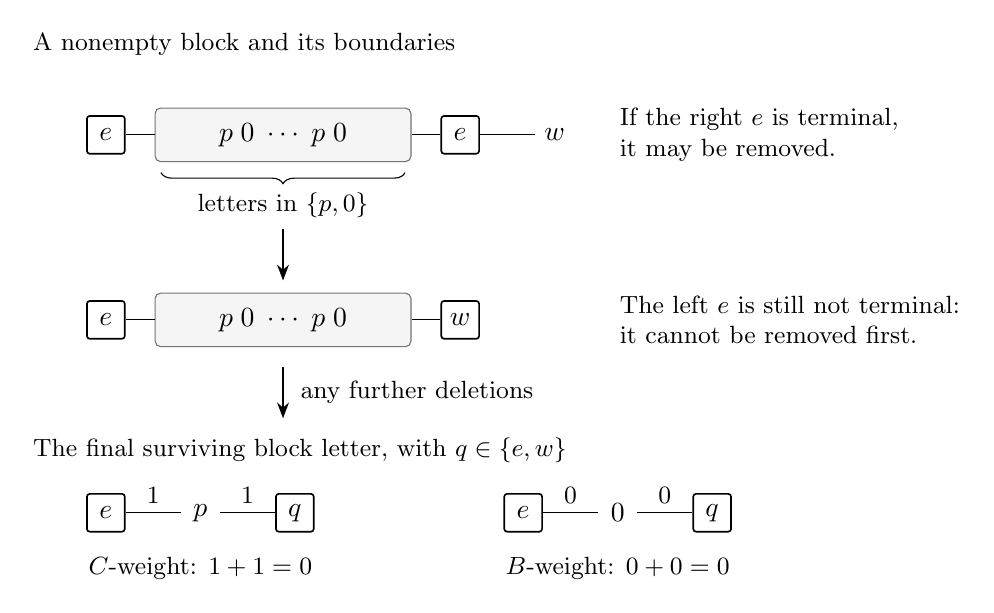
\begin{tikzpicture}[
    x=1cm,y=1cm,
    letter/.style={minimum width=.48cm,minimum height=.48cm,inner sep=1pt},
    boundary/.style={letter,draw,line width=.6pt,rounded corners=1pt},
    block/.style={draw=black!55,fill=black!4,rounded corners=2pt,
      minimum width=3.25cm,minimum height=.68cm,inner sep=3pt},
    move/.style={-{Stealth[length=2mm]},line width=.65pt},
    note/.style={font=\small,align=center,inner sep=2pt}
  ]
    \node[note,anchor=west] at (-5.7,1.15)
      {A nonempty block and its boundaries};
    \node[boundary] (left) at (-4.7,0) {$e$};
    \node[block] (word) at (-2.45,0) {$p\;0\;\cdots\;p\;0$};
    \node[boundary] (right) at (-.2,0) {$e$};
    \node[letter] (end) at (1.0,0) {$w$};
    \draw (left) -- (word) -- (right) -- (end);
    \draw[decorate,decoration={brace,amplitude=4pt,mirror}]
      (-4.0,-.48) -- (-.9,-.48)
      node[note,midway,below=5pt] {letters in $\{p,0\}$};
    \node[note,align=left,anchor=west] at (1.75,0)
      {If the right $e$ is terminal,\\it may be removed.};

    \draw[move] (-2.45,-1.2) -- (-2.45,-1.85);
    \node[boundary] (leftnext) at (-4.7,-2.35) {$e$};
    \node[block] (wordnext) at (-2.45,-2.35) {$p\;0\;\cdots\;p\;0$};
    \node[boundary] (rightnext) at (-.2,-2.35) {$w$};
    \draw (leftnext) -- (wordnext) -- (rightnext);
    \node[note,align=left,anchor=west] at (1.75,-2.35)
      {The left $e$ is still not terminal:\\it cannot be removed first.};

    \draw[move] (-2.45,-2.95) -- (-2.45,-3.6)
      node[note,midway,right=4pt] {any further deletions};
    \node[note,anchor=west] at (-5.7,-4.0)
      {The final surviving block letter, with $q\in\{e,w\}$};

    \node[boundary] (ep) at (-4.7,-4.8) {$e$};
    \node[letter] (p) at (-3.5,-4.8) {$p$};
    \node[boundary] (qp) at (-2.3,-4.8) {$q$};
    \draw (ep) -- node[above,font=\small] {$1$} (p)
      -- node[above,font=\small] {$1$} (qp);
    \node[note] at (-3.5,-5.5) {$C$-weight: $1+1=0$};

    \node[boundary] (ez) at (.6,-4.8) {$e$};
    \node[letter] (zero) at (1.8,-4.8) {$0$};
    \node[boundary] (qz) at (3.0,-4.8) {$q$};
    \draw (ez) -- node[above,font=\small] {$0$} (zero)
      -- node[above,font=\small] {$0$} (qz);
    \node[note] at (1.8,-5.5) {$B$-weight: $0+0=0$};
  \end{tikzpicture}
  \caption{The obstruction in the second summand of the leading pentagon,
  after the minimal $A$-count forces every $e$ to be removed by an
  $A$-operation. Such an operation removes only a terminal $e$.
  While the displayed $p,0$ block is nonempty, its left boundary remains
  $e$; removing a terminal right boundary changes $e$ to $w$.
  With either right boundary, the final surviving $p$ or $0$ has deletion weight
  zero in $\mathbb F_2$. Thus no nonzero deletion sequence empties the block.}
  \label{fig:deletion-block}
\end{figure}


The scalar leading pentagon now gives $[s']\chi_h=0$ for every such
$s$.  The only remaining words have the form $v e^h$, with $v$ a word
of $p$'s and zeros.  Because $m-h>0$, the word $v$ is nonempty.  Let
$\operatorname{rev}$ denote reversal of associative words.  For every
ordinary homogeneous Lie polynomial $q$ of associative length $d$,
\[
 \operatorname{rev}(q)=(-1)^{d-1}q.
\]
Indeed reversal sends $[q_1,q_2]$ to
$-[\operatorname{rev}(q_1),\operatorname{rev}(q_2)]$, proving the
formula by induction on Lie monomials.  In characteristic two it fixes
$\chi_h$.  The coefficient of $v e^h$ therefore equals the coefficient
of $e^h\operatorname{rev}(v)$, which has already been shown to vanish.
Every coefficient of $\chi_h$ is zero, a contradiction.

Thus a least nonzero $A$-count can only be $m$.  All $A$-counts are at
most $m$, so only the component using $A,B$ remains.  It is an ordinary
Lie polynomial as asserted.
\end{proof}

\subsection{Excluding the residual kernel}
Deletion has reduced the possible kernel to polynomials $P(A,B)$.
To exclude them, we now use the special identity rather than further
deletion tests.  Its lowest-count part compares coefficients obtained
by exchanging an $A$ and a $B$; antisymmetry will handle the remaining
case with only one $A$.

\begin{proposition}\label{prop:projection-injective}
For $n>2$ and every $r\geq0$, the leading projection
\[
 \operatorname{gr}^{r}\overline L_n\longrightarrow
 \Lie_{\F}\langle C,B\rangle,\qquad
 \chi\longmapsto\chi(0,C,B)
\]
is injective.  Its source is zero unless $n=2m+r$ for an integer
$m\geq0$; in that case its image has $C$-count $m$ and $B$-count $r$.
\end{proposition}

\begin{proof}
The map is well defined because changing a representative by an
element of $F^{r+1}$ does not change its count-$r$ component.  The
parity assertion and the multidegree of its image follow from
$\wt(A)=\wt(C)=2$ and $\wt(B)=1$.  If $m=0$, the leading part is an ordinary Lie polynomial
in $B$ alone and is zero in the weights at issue.  We may therefore
assume $m>0$.

Suppose that $\chi(0,C,B)=0$.  By Lemma~\ref{lem:deletion-kernel},
$\chi=P(A,B)$.  If $r=0$, this is an ordinary Lie polynomial in $A$
alone, and hence zero except possibly in weight two.  Thus a nonzero
kernel would require $r\geq1$.

Apply the reduction of Lemma~\ref{lem:special} and antisymmetry with
$z=x+y$.  They give
\begin{equation}\label{eq:deletion-special}
 [x,\bar\psi(x,y)+\bar\psi(z,y)]+[y,\bar\psi(z,y)]=0.
\end{equation}
Indeed the special identity with $a=x$, $b=y$, $c=z$ becomes
$[x,\bar\psi(y,x)]+[z,\bar\psi(y,z)]=0$, and antisymmetry in
characteristic two interchanges each pair of arguments.

Under $x\mapsto x+y$, the three associative elements become
\[
 A\mapsto A+C+B^2,\qquad C\mapsto C,\qquad B\mapsto B.
\]
Moreover, on their free associative algebra,
\[
 [x,A]=0,\qquad [x,B]=C,\qquad [x,C]=[A,B].
\]
The part of $\ad_x$ that lowers $B$-count by one is consequently the
derivation
\[
 D(A)=D(C)=0,\qquad D(B)=C;
\]
its other part raises $B$-count by one.  The substitution
$A\mapsto A+C+B^2$ never lowers that count.  Therefore components of
$\bar\psi$ with count greater than $r$ cannot contribute to count
$r-1$ in \eqref{eq:deletion-special}, and its outside bracket with $y$
has count at least $r+1$.  Within the leading part, using any $B^2$
in the substitution also raises the count by two.  The count-$r-1$
component of \eqref{eq:deletion-special} is exactly
\begin{equation}\label{eq:residual-kernel-identity}
 D\bigl(P(A+C,B)+P(A,B)\bigr)=0.
\end{equation}

Write $c(v)$ for the coefficient of a word $v$ with $m$ letters $A$
and $r$ letters $B$ in $P$.  Fix any target word with $m-1$ letters
$A$, $r-1$ letters $B$, and two letters $C$.  Its coefficient on the
left of \eqref{eq:residual-kernel-identity} is the sum of exactly two
coefficients of $P$: fill the two marked $C$-positions with $(A,B)$
or with $(B,A)$.  In each case the original $A$ is replaced by $C$
in the substitution and the original $B$ by $C$ under $D$; these are
the only possibilities.  The term $D(P(A,B))$ has only one $C$ and
contributes nothing here.  Thus the coefficients of $P$ are invariant
under exchanging any chosen $A$-position and $B$-position.  These
exchanges connect all words with the specified multiplicities, so
\begin{equation}\label{eq:constant-residual-coefficients}
 c(v)=\lambda\quad\text{for every such word }v
\end{equation}
for one $\lambda\in\F$.

If $m\geq2$, fix a target word with $m-2$ letters $A$, $r-1$ letters
$B$, and three letters $C$.  Exactly one of its three $C$-positions
must have been the $B$ differentiated by $D$; the other two must have
been $A$'s replaced in the substitution.  There are exactly three
choices.  Its coefficient is therefore $3\lambda=\lambda$, which
\eqref{eq:residual-kernel-identity} forces to vanish.  Hence $P=0$.

It remains to consider $m=1$.  The polynomial $P$ has original
$(x,y)$-bidegree $(2,r)$.  An $A,C,B$ word with counts $(a,c,b)$ has
original bidegree $(2a+c,c+b)$.  Solving for bidegree $(2,r)$ gives
only
\[
 (a,c,b)=(1,0,r)\quad\text{or}\quad(0,2,r-2).
\]
The latter possibility is excluded by the assumption
$\bar\psi\in F^r$, and the former is precisely $P$.  Thus if $P\ne0$,
the entire bidegree-$(2,r)$ component of $\bar\psi$ is nonzero.
Symmetry under $x\leftrightarrow y$ forces a nonzero component of
bidegree $(r,2)$.  Its $B$-count is at most its $y$-count, namely two,
so $F^r$ forces $r\leq2$.

For $r=2$, the ordinary free Lie component with one $A$ and two $B$'s
is spanned by
\[
 [B,[A,B]]=ABB+BBA.
\]
To see the spanning assertion directly, every three-letter bracketing
with two identical $B$'s either has the inner bracket $[B,B]=0$, or
is $[B,[A,B]]$ up to sign and skew-symmetry.  The coefficients on
$ABB,BAB,BBA$ are therefore $(\mu,0,\mu)$, which are all equal as
required by \eqref{eq:constant-residual-coefficients} only when
$\mu=0$.

For $r=1$, the forced swapped bidegree is $(1,2)$.  The count equations
$2a+c=1$, $c+b=2$ have the unique nonnegative solution
$(a,c,b)=(0,1,1)$.  Thus this nonzero component is a multiple of
$[C,B]$, lies in count one, and survives the projection $A=0$.
No higher-filtration component has this bidegree, so it cannot cancel
this projection.  This contradicts $\chi(0,C,B)=0$.  Both exceptional
cases are excluded, proving injectivity.
\end{proof}

\section{The image of the leading projection}
\label{sec:image}

Throughout this section the coefficient field is $\F$.
Recall that $\overline L_n$ denotes the reduction of the saturated
$\Z_{(2)}$-lattice of rational solutions of weight $n$, and that
$F^r$ consists of polynomials containing at least $r$ occurrences of $B$
in the free associative algebra on
\[
 A=x^2,\qquad C=[x,y],\qquad B=y.
\]
We use the ordinary free Lie algebra on $A,C,B$ inside this associative
algebra, as justified in Lemma~\ref{lem:abc-free}.
For $\psi\in F^r\overline L_n$, let $\chi(A,C,B)$ be its component
with exactly $r$ occurrences of $B$, and put
\[
 f(C,B)=\chi(0,C,B).
\]
If this component is nonzero, then $n=2m+r$, where $m$ is the total
number of $A$'s and $C$'s in $\chi$.
Proposition~\ref{prop:projection-injective} says that this projection
is injective on the corresponding associated graded space.
We shall identify a free Lie algebra containing its image.

The argument begins with a restriction on products of iterated adjoints,
obtained from symmetry in $x,y$ in Lemma~\ref{lem:even-indices}.
This restriction gives invariance under the polynomial shifts
$B\mapsto B+s(C)$, and a Vandermonde argument then places $f$ in the
ordinary free Lie algebra generated by $\ad_C^kB$, $k\geq1$.
This proves the all-weight dimension bound.  We then establish a
separate compatibility: projected leading Ihara brackets become
ordinary brackets.  It will provide the independent Hall words in
Section~\ref{sec:induction}.

\subsection{Symmetry and polynomial shifts}

\begin{lemma}[The even-index bound]
\label{lem:even-indices}
Suppose that $n>2$, $\psi\in F^r\overline L_n$, and $n=2m+r$.
The component of $\psi$ of original $(x,y)$-bidegree $(m,m+r)$
is an associative linear combination of products
\begin{equation}
 \label{eq:swapped-products}
 (\ad_y^{j_1}x)\cdots(\ad_y^{j_m}x)
\end{equation}
in which at least $r$ of the indices $j_1,\ldots,j_m$ are even,
with zero counted as even.
Its image under $A=0$ is exactly $f(C,B)$.
In particular, if $r>m$, then $f=0$.
\end{lemma}

\begin{proof}
By the elimination argument in Lemma~\ref{lem:abc-free}, every
homogeneous Lie polynomial in $x,y$ of weight greater than one is a
Lie polynomial in $U_j=\ad_x^j y$, $j\geq0$.
In characteristic two these elimination letters are
\[
 U_{2i}=E_i=\ad_A^i B,
 \qquad
 U_{2i+1}=O_i=\ad_A^i C.
\]
Associative words in the $E_i,O_i$ are linearly independent.
Indeed, order the letters with $A$ largest and use degree followed
by lexicographic order.  The leading words of these letters are
$A^iB,A^iC$, respectively, with coefficient one.
They form a prefix code: one reads a string of $A$'s up to its
next $B$ or $C$, thereby determining each successive codeword.
Distinct products consequently have distinct leading words.

Each $E_i$ is homogeneous of $B$-count one, whereas each $O_i$
has $B$-count zero.  Thus the expansion of $\psi$ in independent
associative words in this alphabet is graded by the number of
$E$-factors.  The hypothesis $\psi\in F^r$ forces the coefficients
of all words with fewer than $r$ such factors to vanish separately.
This establishes a termwise restriction before any substitution
or quotient is taken.

Select the component of original bidegree $(m+r,m)$.
Every $U_j$ has exactly one $y$, so every product in this component
has exactly $m$ factors.  The reduced antisymmetry equation gives
$\psi(x,y)=\psi(y,x)$.  Swapping $x$ and $y$ therefore gives
the desired expression~\eqref{eq:swapped-products} for bidegree
$(m,m+r)$, with the same lower bound on the number of even indices.
If $r>m$, no such product exists.

For completeness, an $A,C,B$-word with respective counts $(a,c,b)$
has original bidegree $(2a+c,c+b)$.  In bidegree $(m,m+r)$ this means
\begin{equation}
 \label{eq:bidegree-counts}
 c=m-2a,\qquad b=r+2a.
\end{equation}
The terms with $a>0$ have higher $B$-count and vanish under $A=0$;
the terms with $a=0$ have $c=m,b=r$ and are precisely $f$.
Thus the even-index bound applies to the whole bidegree component,
including every term subsequently removed by the projection.
\end{proof}

\begin{lemma}[Polynomial shift invariance]
\label{lem:shift-invariance}
For every $f$ obtained as above and every polynomial $s(C)$,
\begin{equation}
 \label{eq:polynomial-shift}
 f(C,B+s(C))=f(C,B).
\end{equation}
The identity holds after adjoining any finite collection of
commuting scalar indeterminates to the coefficients; in particular,
it is a polynomial identity in the coefficients of $s$.
\end{lemma}

\begin{proof}
Let $R$ be any commutative $\F$-algebra, and work in
$S=R\langle C,B\rangle$.  Define an $R$-linear derivation $D$ by
\[
 DB=C,\qquad DC=0.
\]
In characteristic two the square of a derivation is again a
derivation: the two middle terms in the twice-applied product rule
cancel.  Since $D^2$ vanishes on $B,C$, it vanishes on all of $S$.
Consequently the Ore extension, followed by the indicated quotient,
\[
 \mathcal E=S[X;D]/(X^2),\qquad Xq=qX+Dq\quad(q\in S),
\]
has underlying left $S$-module $S\oplus SX$.
Indeed $X^2q=qX^2+D^2q=qX^2$, so $X^2$ is central in the Ore
extension and its quotient introduces no relation in $S$.
In particular, $S$ embeds in $\mathcal E$.
The substitutions $x\mapsto X$, $y\mapsto B$ give
\[
 x^2\mapsto0,\qquad [x,y]\mapsto C.
\]
Equivalently, $\mathcal E$ acts on $S$ with $X$ acting by $D$
and elements of $S$ acting by left multiplication.
For an element written $q+q'X$, its value on $1$ is its constant
term $q$.

Fix $s\in R[C]$, and put $F=B+s(C)$.
The substitution $B\mapsto F$, $C\mapsto C$ commutes with $D$,
since $D(s)=0$.  It therefore extends to an automorphism of
$\mathcal E$ fixing $X$.
Let $h(x,y)$ be the whole bidegree-$(m,m+r)$ component in
Lemma~\ref{lem:even-indices}.  Evaluation at $x=X,y=B$ kills the
terms containing $A$ in its $A,C,B$ expression, so that
$h(X,B)=f(C,B)$ in the embedded subalgebra $S$ of $\mathcal E$.
Applying the shift automorphism just constructed gives
$h(X,F)=f(C,F)$.  We may therefore evaluate the even-index product
expansion of $h$ term by term in $\mathcal E$.  Its sum belongs to
$S$, so its value on $1$ is exactly $f(C,F)$.
The factors of positive index become elements of $S$:
\[
 \ad_F^jX=P_j:=\ad_F^{j-1}C\quad(j\geq1),
\]
whereas the index-zero factor is $X$.
We shall bound the $B$-degree of the constant term of each product
separately.

Write
\[
 L=\ad_B,\qquad Q=\ad_{s(C)},\qquad K=\ad_C,
 \qquad P_j=(L+Q)^{j-1}C.
\]
Here $L$ raises $B$-degree by one and $Q$ preserves it.
The relations needed below are
\[
 Q(C)=0,\qquad QK=KQ,\qquad DL=LD+K,\qquad DQ=QD.
\]
For the two smallest positive indices one has
\begin{equation}
 \label{eq:small-indices}
 P_1=C,\quad DP_1=0,\qquad
 P_2=[B,C],\quad DP_2=0.
\end{equation}
For $j\geq2$, every nonzero operator word in $(L+Q)^{j-1}C$
has rightmost operator $L$, because $Q(C)=0$.
Thus $P_j$ has no $B$-degree-zero component, and its degree-one
component is
\[
 (P_j)_{[1]}=Q^{j-2}LC.
\]
This is killed by $D$, since $DLC=KC=[C,C]=0$.
As $D$ lowers $B$-degree by one, $DP_j$ has no degree-zero
component for any $j\geq1$.

For $j\geq3$, the degree-two component is explicitly
\[
 (P_j)_{[2]}=
 \sum_{a+b=j-3}Q^aLQ^bLC.
\]
Upon applying $D$, differentiating the rightmost $L$ gives zero,
and differentiating the other $L$ gives $Q^aKQ^bLC$.
The commutation of $Q$ and $K$ therefore gives
\begin{equation}
 \label{eq:differentiated-linear-part}
 (DP_j)_{[1]}=(j-2)Q^{j-3}KLC.
\end{equation}
For even $j$ this is zero in $R$.
Together with~\eqref{eq:small-indices}, these calculations prove
the following lower bounds; the zero polynomial satisfies every
listed bound:
\[
\begin{array}{c|cc}
 & P_j & DP_j\\ \hline
 j\geq1\text{ odd} & 0 & 1\\
 j\geq2\text{ even} & 1 & 2
\end{array}
\qquad\text{(minimum $B$-degree).}
\]
The bound for odd $P_j$ is deliberately weak, so that it includes
$P_1=C$.
All these calculations allow constant terms in $s$ and arbitrary
scalar coefficients in $R$.

Now consider one product with $q$ index-zero factors and $e$ positive
even-index factors.  Move each $X$ to the right using
$XP=PX+DP$, and apply the resulting expression to $1$.
Every surviving term must use each of the original $q$ copies of
$X$ as a differentiation, since a terminal $X$ kills $1$.
Repeated use of the product rule assigns these differentiations
to positive-index factors to their right.  An allocation assigning
two differentiations to the same factor vanishes, because $D^2=0$.
Hence every surviving term is a product in which exactly $q$
distinct positive-index factors have been differentiated once.
An undifferentiated positive even-index factor contributes a lower
bound of one, and an odd-index factor contributes a lower bound
of zero.  Differentiating either type increases the respective
lower bound by one.  The resulting $B$-degree is therefore at least
\[
 e+q,
\]
which is precisely the number of all even indices, including zero.
If no such allocation is possible the constant term is zero, which
also satisfies the bound.  Cancellations among allocations cannot
create lower-degree terms.

Lemma~\ref{lem:even-indices} now shows that $f(C,B+s(C))$ has no
$B$-degree below $r$.  On the other hand, $f$ is homogeneous of
$B$-degree $r$, and replacing $B$ by $B+s(C)$ cannot increase that
degree.  Its degree-$r$ component is exactly $f(C,B)$, obtained by
choosing $B$ at every occurrence.  This proves
\eqref{eq:polynomial-shift} over $R$, and in particular over any
polynomial ring in scalar indeterminates.
\end{proof}

\subsection{The ordinary Lie image and the dimension bound}
\begin{proposition}[The image bound]
\label{prop:image-bound}
Set $g_k=\ad_C^kB$ for $k\geq1$.
These elements freely generate an ordinary free Lie algebra inside
$\Lie_{\F}\langle C,B\rangle$.
For $n>2$, the image of the leading projection of
$\operatorname{gr}^r_F\overline L_n$ belongs to its weight-$n$,
length-$r$ component, where $\wt(g_k)=2k+1$ and each $g_k$ has
length one.
The associated graded piece with $r=0$ is zero.
\end{proposition}

\begin{proof}
First suppose $r\geq1$.
Encode the associative words of $B$-degree $r$ by the vector-space
isomorphism
\[
 \mathcal P_r:
 C^{i_0}BC^{i_1}\cdots BC^{i_r}
 \longmapsto s_0^{i_0}s_1^{i_1}\cdots s_r^{i_r}
 \quad\text{in }\F[s_0,\ldots,s_r].
\]
Put $P=\mathcal P_r(f)$.
For $1\leq i\leq r$, let $R_iP$ be its restriction obtained by
identifying $s_{i-1}$ and $s_i$, written in the same polynomial
ring $\F[t_0,\ldots,t_{r-1}]$ for every $i$:
\[
 R_iP=P(t_0,\ldots,t_{i-2},t_{i-1},t_{i-1},
               t_i,\ldots,t_{r-1}).
\]
Empty initial or final strings in this formula are omitted.
In the coefficient of $\lambda$ in $f(C,B+\lambda C^j)$, replacing
the $i$th $B$ merges its two neighboring powers of $C$ and adds
$j$ to their exponent.  Its encoding with $r-1$ remaining $B$'s
is consequently $t_{i-1}^{j}R_iP$.
Lemma~\ref{lem:shift-invariance}, applied with the independent
scalar $\lambda$, gives
\begin{equation}
 \label{eq:vandermonde-system}
 \sum_{i=1}^r t_{i-1}^{j}R_iP=0\qquad(j\geq0).
\end{equation}
Taking $j=0,\ldots,r-1$ produces a Vandermonde matrix whose
determinant is
\[
 \prod_{0\leq a<b\leq r-1}(t_b-t_a).
\]
It is a nonzero polynomial over $\F$, because the $t_i$ are
independent indeterminates.  Thus the matrix is invertible over
$\F(t_0,\ldots,t_{r-1})$, and all $R_iP$ vanish.
This argument also applies to even $r$; it never divides by $r$
or specializes the $t_i$ to elements of the two-element field.
For $r=1$ the matrix is simply $(1)$.

The kernel of the $i$th identification is the principal ideal
generated by $d_i=s_{i-1}-s_i$.
These $d_i$ are distinct nonassociate prime linear polynomials.
Their individual divisibility therefore implies
\begin{equation}
 \label{eq:consecutive-divisibility}
 d_1\cdots d_r\mid P
 \quad\text{in }\F[s_0,\ldots,s_r].
\end{equation}
It remains to translate this associative statement into an
ordinary Lie statement.

Temporarily include $g_0=B$.
The ordinary Lie ideal generated by $B$ in
$\Lie_{\F}\langle C,B\rangle$ is the subalgebra generated by
$g_k=\ad_C^kB$, $k\geq0$.
Indeed, this subalgebra contains $B$ and is stable under $\ad_C$
by the derivation rule and $[C,g_k]=g_{k+1}$; the reverse inclusion
is immediate.  Since $f$ has positive $B$-degree, it belongs to
this ordinary Lie subalgebra.

Expanding the iterated adjoints gives the useful product formula
\begin{equation}
 \label{eq:gap-monomials}
 \mathcal P_r(g_{k_1}\cdots g_{k_r})
 =\prod_{i=1}^r(s_{i-1}-s_i)^{k_i}
 =d_1^{k_1}\cdots d_r^{k_r}.
\end{equation}
The variables $d_1,\ldots,d_r,s_r$ are an invertible linear
change of coordinates from $s_0,\ldots,s_r$.
In particular, the monomials in the right side of
\eqref{eq:gap-monomials} are linearly independent.
For different product lengths the $B$-degrees differ, so all
associative words in the $g_k$, $k\geq0$, are independent.
Their ordinary Lie algebra is therefore the ordinary free Lie
algebra on these letters, by its embedding in the free associative
algebra.

Write the associative expansion of $f$ uniquely in these independent
words.  Its encoding lies in $\F[d_1,\ldots,d_r]$.
By~\eqref{eq:consecutive-divisibility}, every monomial appearing
with nonzero coefficient has positive exponent of every $d_i$.
Equivalently, the expansion of $f$ contains no word with any factor
$g_0$.  The ordinary free Lie algebra on $g_0,g_1,\ldots$ has a
retraction
\[
 \rho(g_0)=0,\qquad \rho(g_k)=g_k\quad(k\geq1).
\]
Its extension to the free associative algebra fixes the expansion
of $f$.  Hence $\rho(f)=f$, proving that $f$ belongs to the
ordinary free Lie algebra on $g_k$, $k\geq1$.
This retraction preserves ordinary Lie membership throughout;
no identification with all primitive elements in characteristic
two is being made.

Each $g_k$ contains one $B$ and $k$ copies of $C$.
The original weight is therefore $2k+1$, and the $B$-count of a
Lie word is its length in these generators.  This proves the
asserted weight and length statement.

If $r=0$, then $f$ is an ordinary Lie polynomial in $C$ alone.
The ordinary Lie algebra on one generator is its one-dimensional
linear span, of original weight two; thus $f=0$ for $n>2$.
Proposition~\ref{prop:projection-injective} then gives
$\operatorname{gr}^0_F\overline L_n=0$.
The possible boundary $m=0$ also contributes nothing: its leading
component would be an ordinary Lie polynomial in $B$ alone,
whose only possible positive weight is one.
\end{proof}

Define the ordinary free Lie algebra
\[
 \mathfrak f_{\mathrm{odd}}
   =\Lie_{\F}\langle z_k:k\geq1\rangle,
 \qquad \wt(z_k)=2k+1,
\]
and give each $z_k$ length one.
Write $\mathfrak f_{\mathrm{odd},n,r}$ for its component of
weight $n$ and length $r$, and set
\begin{equation}
 \label{eq:free-dimensions}
 d_{n,r}=\dim_{\F}\mathfrak f_{\mathrm{odd},n,r},
 \qquad d_n=\sum_{r\geq0}d_{n,r}.
\end{equation}
These are also the corresponding dimensions over $\Q$, by
the ordinary free Lie lattice of Lemma~\ref{lem:lie-lattice}.
The sum is finite: a length-$r$ word has weight at least $3r$,
and only finitely many generators can occur in any fixed weight.

\begin{corollary}[The all-weight upper bound]
\label{cor:dimension-bound}
For every $n$ and $r\geq0$ there is an injection
\[
 \operatorname{gr}^r_F\overline L_n
 \lhook\joinrel\longrightarrow
 \mathfrak f_{\mathrm{odd},n,r},
\]
obtained by the leading projection and the identification
$g_k\leftrightarrow z_k$.  In particular,
\begin{equation}
 \label{eq:dimension-upper-bound}
 \dim_{\Q}W_n
 =\dim_{\F}\overline L_n
 \leq\sum_{r\geq0}d_{n,r}=d_n.
\end{equation}
\end{corollary}

\begin{proof}
For $n>2$, combine Proposition~\ref{prop:projection-injective}
with Proposition~\ref{prop:image-bound}.
If $n-r$ is odd or negative the source piece is zero by the
weights of $A,C,B$, and the target piece is likewise zero since
the weight of a length-$r$ word in odd-weight letters has parity
$r$.  The cases $r=0$ and $m=0$ were disposed of in
Proposition~\ref{prop:image-bound}.
Weights one and two have zero solution space by
Lemma~\ref{lem:low-weights}, and have no generators or Lie words
in $\mathfrak f_{\mathrm{odd}}$.
Finally, $F^{n+1}\overline L_n=0$, so this is a finite filtration
in weight $n$ and the dimensions of its associated graded pieces
sum to $\dim_{\F}\overline L_n$.
The equality of this dimension with $\dim_{\Q}W_n$ is
Proposition~\ref{prop:saturated-reduction}.
\end{proof}

\subsection{Leading Ihara brackets}
The upper bound concerns the full equation space.  To attain it in
Section~\ref{sec:induction}, we will construct elements whose projected
leading terms are the $g_k$ and compare their iterated Ihara brackets
with ordinary Lie words.  The following compatibility is computed in
the ambient Lie algebra and does not require closure of $W$.

\begin{proposition}[The leading Ihara bracket]
\label{prop:leading-ihara}
Let $\psi\in F^r\overline L_n$ and
$\phi\in F^s\overline L_{n'}$, where $n,n'>2$ and $r,s\geq1$.
Write $f,g$ for their leading projections at counts $r,s$.
Their Ihara bracket, computed in the ambient Lie algebra in
$x,y$, belongs to $F^{r+s}$ in the $A,C,B$ presentation, and
the projection of its component of count $r+s$ is
\begin{equation}
 \label{eq:leading-ihara}
 [f,g].
\end{equation}
This assertion does not require prior closure of the full solution
space under the Ihara bracket.
\end{proposition}

\begin{proof}
We first prove the filtration assertion before applying $A=0$.
The derivation $\delta=\ad_x$ acts on the free $A,C,B$ algebra by
\[
 \delta A=0,\qquad \delta B=C,\qquad \delta C=[A,B].
\]
Write $\delta=\delta_-+\delta_+$, where
\[
 \delta_-B=C,\quad \delta_-A=\delta_-C=0,
 \qquad
 \delta_+C=[A,B],\quad \delta_+A=\delta_+B=0.
\]
These two derivations respectively lower and raise the $B$-count
by one.  In particular, $\delta(F^r)\subset F^{r-1}$.
Directly from the definition of the Ihara derivation,
\begin{equation}
 \label{eq:ihara-abc-action}
 D_\psi A=0,\qquad
 D_\psi B=[B,\psi],\qquad
 D_\psi C=[C,\psi]+[B,\delta\psi].
\end{equation}
The last formula is the derivation identity applied to $[x,B]$.
Thus $D_\psi B\in F^{r+1}$ and $D_\psi C\in F^r$:
the outside $B$ in $[B,\delta\psi]$ restores the one count that
$\delta_-$ can remove.  Replacing a $B$ in a word of count $s$
adds at least $r$ to its count, and replacing a $C$ also adds at
least $r$; the derivative of an $A$ vanishes.
It follows that
\[
 D_\psi(F^s)\subset F^{r+s}.
\]
Interchanging $\psi,\phi$ and including their ordinary bracket
proves the asserted containment of the Ihara bracket.

Let $\chi,\eta$ be the components of $\psi,\phi$ of counts
$r,s$.  In~\eqref{eq:ihara-abc-action}, only $\chi$ can contribute
to the part of the derivation that raises count by exactly $r$.
Its action is
\[
 A\longmapsto0,\qquad
 B\longmapsto[B,\chi],\qquad
 C\longmapsto[C,\chi]+[B,\delta_-\chi].
\]
Indeed, a higher-count component of $\psi$ still has higher count
after applying $[B,\delta_-(-)]$, while
$[B,\delta_+\chi]$ raises the count by two more.
This derivation preserves the ideal generated by $A$, so it
descends under $A=0$.
The projection commutes with $\delta_-$, whose induced action
on $\F\langle C,B\rangle$ is the derivation $D$ from
Lemma~\ref{lem:shift-invariance}.
The induced leading action is consequently
\[
 B\longmapsto[B,f],\qquad
 C\longmapsto[C,f]+[B,Df].
\]
By Proposition~\ref{prop:image-bound}, $f$ is an ordinary Lie
polynomial in $g_k$, $k\geq1$; each of these is killed by $D$,
because
\[
 Dg_k=\ad_C^k(C)=0\quad(k\geq1).
\]
Thus the extra term $[B,Df]$ vanishes, and the induced derivation
on $\F\langle C,B\rangle$ is $q\mapsto[q,f]$.
One can also read $Df=0$ directly as the coefficient of $\lambda$
in~\eqref{eq:polynomial-shift} with $s(C)=\lambda C$.

The two Ihara derivations therefore project to $[g,f]$ and
$[f,g]$, respectively, and the ordinary bracket projects to
$[f,g]$.  Their specified combination is
\[
 [g,f]-[f,g]+[f,g]=[g,f]=[f,g]
\]
over $\F$.
All higher components of $\psi$ or $\phi$ have already been
excluded by the filtration calculation, so this proves
\eqref{eq:leading-ihara}.
\end{proof}

\section{A rational Lie algebra of categorical values}\label{sec:category}

The upper bound on the full equation space is now established.  To
attain it, we construct a rational subspace that is closed under the
Ihara bracket and contains an element with nonzero coefficient of
$x^{n-1}y$ in every odd weight $n\geq3$.  This section proves the
closure property; the next constructs the nonzero values.
Only configurations with at most four labels will be needed.
We use the parenthesized-chord formalism of Bar-Natan
\cite[Sections~2--3]{BarNatan}, restricted to the finite arities and
operations specified below.
All completions in this section are by weight, and all tensor products of
completed spaces are completed by total weight.

We use the standard label sets $[k]=\{1,\ldots,k\}$ for
$1\leq k\leq4$; other label sets denote their relabeled copies.
For such a finite label set $I$, let
$\mathcal T(I)$ be the set of planar binary trees whose leaves are
bijectively labeled by $I$.  Thus the objects record both parentheses and
a linear ordering.  Put $\mathfrak t_I=0$ for $|I|=1$, and otherwise use
the infinitesimal braid algebra on $I$.  Over a field $K$ of
characteristic zero define a $K$-linear category $\mathcal C(I;K)$ by
\[
 \operatorname{Hom}(p,q)=\widehat U(\mathfrak t_I\otimes K)
 \qquad(p,q\in\mathcal T(I)).
\]
Composition is multiplication, with the last arrow on the left.  Write
$1_{pq}$ for the arrow with coefficient $1$, so that
$1_{qr}1_{pq}=1_{pr}$.  Each arrow space carries the coproduct determined
by
\[
 \Delta(t_{ij})=t_{ij}\otimes1+1\otimes t_{ij},
 \qquad \Delta(1_{pq})=1_{pq}\otimes1_{pq}.
\]
In particular, the unit coefficient arrow between different objects is
distinguished from an identity endomorphism.

Here are all the additional operations that we impose.  Relabeling is
allowed along every bijection of label sets.  For an outer tree on $I$
and fixed trees on disjoint nonempty sets $B_i$, graft the latter at its
leaves.  On arrows this operation is the algebra homomorphism
\begin{equation}\label{eq:category-block-sum}
 t_{ij}\longmapsto t_{B_iB_j}:=
 \sum_{a\in B_i,\ b\in B_j}t_{ab}.
\end{equation}
There is also insertion of a varying tree in one fixed leaf of a fixed
outer tree: on arrows this retains each inner chord $t_{ab}$ with its
labels.  Both operations are used whenever the resulting number of
leaves is at most four; single-leaf trees permit identity insertions.
These are functors preserving coproducts.  Indeed, the disjoint-chord
relations and the three-label relations imply the corresponding
relations between the block sums in
\eqref{eq:category-block-sum}, by summing first over labels in each
block.  Inner chords commute with outer block sums: for
$a,b\in B_i$ and $c\notin B_i$ the only possibly nonzero terms are
$[t_{ab},t_{ac}+t_{bc}]=0$.  These observations also show that successive
insertions agree with grafting the same trees in one step.

A \emph{compatible derivation of weight $n$} is a family $\delta$ of
$K$-linear maps on these arrow spaces, raising weight by $n$, such that
\[
 \delta(ba)=\delta(b)a+b\delta(a),\qquad
 \Delta\delta=(\delta\otimes\id+\id\otimes\delta)\Delta.
\]
It must commute with all the operations just specified and vanish on
all arrow spaces in arity two.  The arity-one derivation is necessarily
zero.  Let $\mathcal D_n(K)$ denote this space.  Commutators of such
families are again compatible derivations, of the sum of their weights.

Set
\[
 a=((12)3),\qquad b=(1(23)),\qquad
 \alpha=1_{ab},\qquad x=t_{12},\quad y=t_{23}.
\]
Evaluation on $\alpha$ will be understood as its coefficient in
$\widehat U(\mathfrak t_3\otimes K)$.

\begin{proposition}\label{prop:categorical-values}
For $n\geq2$, evaluation $\delta\mapsto\delta(\alpha)$ takes
$\mathcal D_n(\Q)$ into $W_n$.  Its images
\[
 V_n=\{\delta(\alpha):\delta\in\mathcal D_n(\Q)\},\qquad
 V=\bigoplus_{n\geq2}V_n,
\]
form a rational Lie subalgebra under the Ihara bracket \eqref{eq:ihara}.
\end{proposition}

\begin{proof}
Write $\psi=\delta(\alpha)$.  The coderivation rule at the group-like
arrow $\alpha$ says
\[
 \Delta\psi=\psi\otimes1+1\otimes\psi.
\]
Primitives in a characteristic-zero enveloping algebra are its Lie
algebra: by the PBW filtration, a primitive of filtration degree
$d>1$ would give a primitive homogeneous polynomial of degree $d$ in a
symmetric algebra, whereas its coproduct has a nonzero component of
bidegree $(1,d-1)$.  Induction on filtration degree proves the assertion.
Now
\begin{equation}\label{eq:category-three-split}
 \mathfrak t_3=\Lie_K\langle x,y\rangle\oplus K T,
 \qquad T=t_{12}+t_{13}+t_{23},
\end{equation}
with $T$ central: replacing $t_{13}$ by $T-x-y$ transforms exactly the
three defining relations into the centrality of $T$.  Thus a primitive
of weight $n\geq2$ is a Lie polynomial $\psi(x,y)$.

Reversing the two children at any fork is insertion, followed if
necessary by an inner insertion, of a unit arrow in arity two.  Its
$\delta$-value is zero.  The values of unit coefficient arrows add under
composition, and inverse unit arrows have opposite values.  Relabel
$\alpha$ by $1\leftrightarrow3$.  Its source $((32)1)$ is carried to $b$
by fork reversals, and its target $(3(21))$ is carried to $a$ in the same
way.  Its value is therefore both $\psi(y,x)$ and $-\psi(x,y)$, giving
\begin{equation}\label{eq:category-antisymmetry}
 \psi(x,y)+\psi(y,x)=0.
\end{equation}
For the cyclic relation, use the successive trees
$((12)3),((23)1),((31)2)$.  Reassociation on the ordered triples
$(1,2,3),(2,3,1),(3,1,2)$, each followed by a root-fork reversal,
forms a cycle of unit arrows.  Consequently
\[
 \psi(t_{12},t_{23})+\psi(t_{23},t_{31})+
 \psi(t_{31},t_{12})=0.
\]
An occurrence of the central $T$ in a Lie monomial of degree greater
than one contributes zero.  Substitution of $t_{31}=T-x-y$ gives
\begin{equation}\label{eq:category-cyclic}
 \psi(x,y)+\psi(y,-x-y)+\psi(-x-y,x)=0.
\end{equation}

Figure~\ref{fig:reassociation} shows the five four-leaf trees and
the two paths of reassociation arrows:
\[
\begin{gathered}
 A=(((12)3)4),\quad B=((1(23))4),\quad C=(1((23)4)),\\
 D=((12)(34)),\qquad E=(1(2(34))),\\
 A\longrightarrow D\longrightarrow E,
 \qquad A\longrightarrow B\longrightarrow C\longrightarrow E.
\end{gathered}
\]
The two edge values on the first path are
$\psi(t_{13}+t_{23},t_{34})$ and
$\psi(t_{12},t_{23}+t_{24})$.  Those on the second are
$\psi(t_{12},t_{23})$,
$\psi(t_{12}+t_{13},t_{24}+t_{34})$, and
$\psi(t_{23},t_{34})$.
Both composites are $1_{AE}$, hence
\begin{equation}\label{eq:category-pentagon}
\begin{split}
 \psi(t_{12},t_{23}+t_{24})+
 \psi(t_{13}+t_{23},t_{34})
 ={}&\psi(t_{23},t_{34})\\
 &+\psi(t_{12}+t_{13},t_{24}+t_{34})
 +\psi(t_{12},t_{23}).
\end{split}
\end{equation}
This proves membership in $W_n$ using only the stated operations.

\begin{figure}[!t]
  \centering
  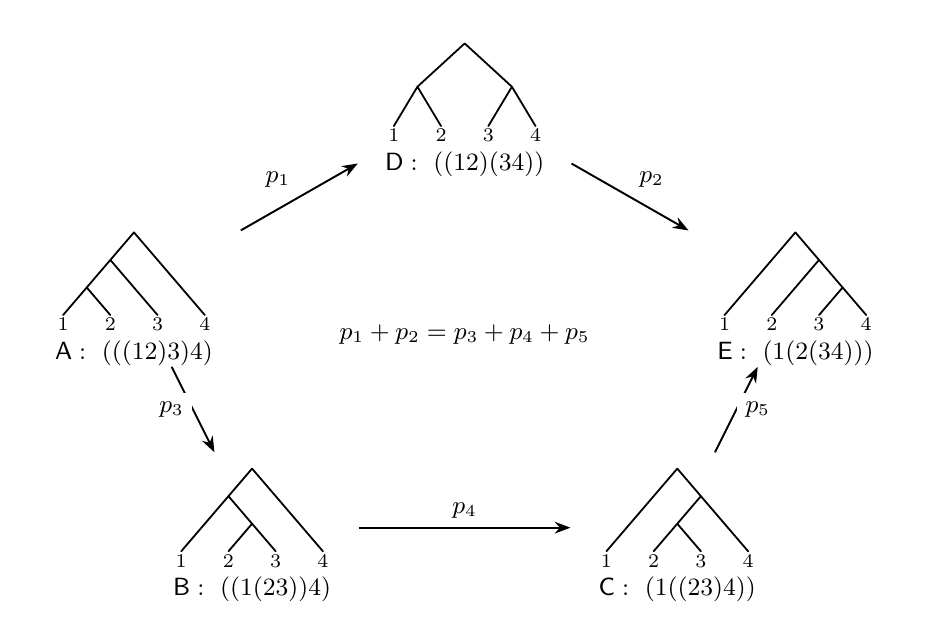
\begin{tikzpicture}[
    x=1cm,y=1cm,
    vertex/.style={minimum width=2.7cm,minimum height=1.9cm,inner sep=0pt},
    tree/.style={line width=.65pt,line cap=round,line join=round},
    reassociate/.style={-{Stealth[length=2mm]},line width=.7pt},
    edge value/.style={fill=white,inner sep=3pt,font=\small},
    leaf/.style={font=\scriptsize,inner sep=1pt},
    tree caption/.style={font=\small,inner sep=1pt}
  ]
    \node[vertex] (A) at (-4.2,0) {};
    \node[vertex] (D) at (0,2.4) {};
    \node[vertex] (E) at (4.2,0) {};
    \node[vertex] (B) at (-2.7,-3) {};
    \node[vertex] (C) at (2.7,-3) {};

    \draw[reassociate] (A) -- node[edge value,above left] {$p_1$} (D);
    \draw[reassociate] (D) -- node[edge value,above right] {$p_2$} (E);
    \draw[reassociate] (A) -- node[edge value,left] {$p_3$} (B);
    \draw[reassociate] (B) -- node[edge value,above] {$p_4$} (C);
    \draw[reassociate] (C) -- node[edge value,right] {$p_5$} (E);

    \begin{scope}[shift={(A)}]
      \draw[tree] (0,.75) -- (-.3,.4) -- (-.6,.05) -- (-.9,-.3)
        (-.6,.05) -- (-.3,-.3) (-.3,.4) -- (.3,-.3)
        (0,.75) -- (.9,-.3);
      \foreach \x/\i in {-.9/1,-.3/2,.3/3,.9/4}
        \node[leaf,below] at (\x,-.3) {$\i$};
      \node[tree caption] at (0,-.78) {$\mathsf{A}:\ (((12)3)4)$};
    \end{scope}
    \begin{scope}[shift={(D)}]
      \draw[tree] (0,.75) -- (-.6,.2) -- (-.9,-.3)
        (-.6,.2) -- (-.3,-.3)
        (0,.75) -- (.6,.2) -- (.3,-.3)
        (.6,.2) -- (.9,-.3);
      \foreach \x/\i in {-.9/1,-.3/2,.3/3,.9/4}
        \node[leaf,below] at (\x,-.3) {$\i$};
      \node[tree caption] at (0,-.78) {$\mathsf{D}:\ ((12)(34))$};
    \end{scope}
    \begin{scope}[shift={(E)}]
      \draw[tree] (0,.75) -- (-.9,-.3)
        (0,.75) -- (.3,.4) -- (-.3,-.3)
        (.3,.4) -- (.6,.05) -- (.3,-.3)
        (.6,.05) -- (.9,-.3);
      \foreach \x/\i in {-.9/1,-.3/2,.3/3,.9/4}
        \node[leaf,below] at (\x,-.3) {$\i$};
      \node[tree caption] at (0,-.78) {$\mathsf{E}:\ (1(2(34)))$};
    \end{scope}
    \begin{scope}[shift={(B)}]
      \draw[tree] (0,.75) -- (-.3,.4) -- (-.9,-.3)
        (-.3,.4) -- (0,.05) -- (-.3,-.3)
        (0,.05) -- (.3,-.3) (0,.75) -- (.9,-.3);
      \foreach \x/\i in {-.9/1,-.3/2,.3/3,.9/4}
        \node[leaf,below] at (\x,-.3) {$\i$};
      \node[tree caption] at (0,-.78) {$\mathsf{B}:\ ((1(23))4)$};
    \end{scope}
    \begin{scope}[shift={(C)}]
      \draw[tree] (0,.75) -- (-.9,-.3)
        (0,.75) -- (.3,.4) -- (0,.05) -- (-.3,-.3)
        (0,.05) -- (.3,-.3) (.3,.4) -- (.9,-.3);
      \foreach \x/\i in {-.9/1,-.3/2,.3/3,.9/4}
        \node[leaf,below] at (\x,-.3) {$\i$};
      \node[tree caption] at (0,-.78) {$\mathsf{C}:\ (1((23)4))$};
    \end{scope}
    \node[align=center,font=\small] at (0,-.55)
      {$p_1+p_2=p_3+p_4+p_5$};
  \end{tikzpicture}

  \smallskip
  {\small
  \begin{tabular}{@{}cl@{\qquad}cl@{}}
    \toprule
    Label & Infinitesimal value & Label & Infinitesimal value \\
    \midrule
    $p_1$ & $\psi(t_{13}+t_{23},t_{34})$
      & $p_3$ & $\psi(t_{12},t_{23})$ \\
    $p_2$ & $\psi(t_{12},t_{23}+t_{24})$
      & $p_4$ & $\psi(t_{12}+t_{13},t_{24}+t_{34})$ \\
    & & $p_5$ & $\psi(t_{23},t_{34})$ \\
    \bottomrule
  \end{tabular}}
  \caption{The five parenthesizations of four ordered leaves. Each arrow
  reassociates $((IJ)K)$ to $(I(JK))$, with the appropriate fixed subtrees
  inserted. The labels $p_1,\ldots,p_5$ denote the infinitesimal values
  in the table, not the arrows themselves.
  The two paths $\mathsf{A}\to\mathsf{D}\to\mathsf{E}$ and
  $\mathsf{A}\to\mathsf{B}\to\mathsf{C}\to\mathsf{E}$ have the same unit
  arrow as composite. Their infinitesimal values add, yielding the pentagon
  identity.}
  \label{fig:reassociation}
\end{figure}


It remains to check the bracket, including its sign.  Let $d_a,d_b$
be the loop derivations at $a,b$.  Inner insertion gives $d_a(x)=0$
and $d_b(y)=0$.  Differentiating the equality of arrows
$\alpha y_a=y_b\alpha$ gives
\[
 \psi y+d_a(y)=y\psi,
 \qquad d_a(y)=[y,\psi].
\]
Outer arity-two insertion also kills $t_{13}+t_{23}$ at $a$, so
$d_a(T)=0$.  In the decomposition
\eqref{eq:category-three-split} its restriction is exactly $D_\psi$.
An arrow from $a$ to $b$ with coefficient $h$ equals $\alpha h_a$;
therefore
\begin{equation}\label{eq:category-arrow-derivative}
 \delta_{ab}(h)=\psi h+D_\psi(h)
 \qquad(h\in K\langle\!\langle x,y\rangle\!\rangle).
\end{equation}
If another derivation $\varepsilon$ has value $\phi$, their commutator
has value
\[
 [\delta,\varepsilon](\alpha)
 =D_\psi(\phi)-D_\phi(\psi)+\psi\phi-\phi\psi
 =\{\psi,\phi\}.
\]
Evaluation is thus a Lie homomorphism onto its image.  No injectivity
of evaluation is required.
\end{proof}

\begin{lemma}[Rational finite data]\label{lem:rational-descent}
For every $n>0$ and every characteristic-zero extension $K/\Q$,
\[
 \mathcal D_n(K)=\mathcal D_n(\Q)\otimes_{\Q}K.
\]
For $n\geq2$, the image of evaluation is $V_n\otimes_{\Q}K$.
In particular, if the coefficient of a fixed associative word is
nonzero on a complex categorical value of weight $n$, it is nonzero
on some rational categorical value of that weight.
\end{lemma}

\begin{proof}
At each arity choose a base object $o$.  For a composition derivation
put $h_p=\delta(1_{op})$, with $h_o=0$, and let $d$ be its derivation on
loops at $o$.  Since every arrow has the factorization
$1_{oq}\,u_o\,1_{po}$, the product and inverse rules force
\begin{equation}\label{eq:category-finite-data}
 \delta_{pq}(u)=h_qu+d(u)-uh_p.
\end{equation}
Conversely, an algebra derivation $d$ and elements $h_p$ define a
composition derivation by this formula.  In weight $n$ the data are
\[
 h_p\in U(\mathfrak t_I)_n,
 \qquad d(t_{ij})\in U(\mathfrak t_I)_{n+1}.
\]
There are finitely many objects and generators, and every displayed
space is finite dimensional over $\Q$.

The conditions that $d$ preserve the defining braid relations are
rational linear equations in these data.  The coderivation conditions
are equivalent to primitivity of all $h_p$ and $d(t_{ij})$: necessity
follows on the reference unit arrows and generator loops, and
sufficiency follows by the product rule and
\eqref{eq:category-finite-data}.  These are again finitely many rational
linear equations, since coproducts in the indicated weights take
values in finite sums of finite-dimensional spaces.

Finally, there are only finitely many label permutations, object
graftings, and inner placements through arity four.  For each associated
functor $\rho$, the condition $\delta\rho=\rho\delta$ need only be
checked on the reference unit arrows and generator loops: all other
arrows follow by composition, the product rule, and continuity.
These checks, and the requirement of zero arity-two action, are
rational linear equations.  Thus $\mathcal D_n$ is the kernel of a
linear map between finite-dimensional rational spaces.  Kernels and
images of such maps commute with scalar extension.  Evaluation and
coefficient extraction are rational linear maps, proving the last
assertion as well.
\end{proof}

\section{Holonomy and odd depth-one values}\label{sec:holonomy}

By Lemma~\ref{lem:rational-descent}, a complex categorical value with
nonzero coefficient of $x^{n-1}y$ gives a rational value with the same
nonvanishing property.  We construct these complex values directly
from a flat connection.
This follows the associator approach to odd-weight elements in
\cite[Proposition~6.3]{Drinfeld}; we include the regularization and
compatibility arguments needed here.  The section first constructs
regularized transport (Proposition~\ref{prop:regularized-holonomy}),
then compares the two transport rules through their operator logarithm,
and finally extracts the nonzero coefficient in
Proposition~\ref{prop:odd-depth-one}.

\subsection{Tree endpoints and regularized transport}
Write $\lambda=(2\pi i)^{-1}$ and
\[
 X_I=\{(z_i)_{i\in I}\in\CC^I:z_i\ne z_j\text{ for }i\ne j\}.
\]
On $X_I$ consider the universal logarithmic braid connection
\cite[Section~1.3]{Kohno}
\begin{equation}\label{eq:holonomy-connection}
 \Omega=\lambda\sum_{i<j}t_{ij}\,d\log(z_i-z_j),
 \qquad dg=\Omega g.
\end{equation}
At every fixed weight this is an ordinary differential equation in a
finite-dimensional nilpotent quotient of the enveloping algebra.
Its solution is the finite sum of iterated integrals in that quotient,
with later differentials multiplying on the left.

The connection is flat.  Its coefficients are closed; terms supported
on four different labels commute; and the remaining terms in
$\Omega\wedge\Omega$ vanish by the three-label braid relations and
\[
 d\log(z_i-z_j)\wedge d\log(z_j-z_k)
 +d\log(z_j-z_k)\wedge d\log(z_k-z_i)
 +d\log(z_k-z_i)\wedge d\log(z_i-z_j)=0.
\]
This is Arnold's logarithmic-form relation \cite{Arnold}.
It follows by putting $u=z_i-z_j$, $v=z_j-z_k$ and using
$z_k-z_i=-u-v$.  The usual homotopy variation formula for an ordinary
differential equation now shows that transport is homotopy invariant:
the variation of transport with fixed endpoints is the integral of
its curvature conjugated by partial transports, and is zero here.
Alternatively this formula follows by differentiating the finite
iterated-integral expression in each weight.
Since $\Omega$ is primitive, transport is group-like.  Indeed its
coproduct and the tensor square of transport solve the same equation
with form $\Omega\otimes1+1\otimes\Omega$ and initial value $1$.

We first define the endpoint data for a fixed choice of scales.
For an internal node $d$ of a tree $p\in\mathcal T(I)$ assign a scale
$s_d=\epsilon^{a_d}$, with $a_{\mathrm{root}}=0$ and exponents strictly
increasing along descent.  Anchor the root at $0$.  The left child of a
node has its anchor at that node's anchor, and the right child has its
anchor displaced by $s_d$; repeat down the tree.  Thus the coordinate
of a leaf is explicitly
\begin{equation}\label{eq:holonomy-tree-coordinate}
 z_i(\epsilon)=
 \sum_{d\text{ above }i}
 \mathbf1_{\{i\text{ lies in the right child of }d\}}\epsilon^{a_d}.
\end{equation}
For sufficiently small positive $\epsilon$ these are distinct real
points in the prescribed leaf order.  The curve
$\epsilon\mapsto(z_i(\epsilon))_{i\in I}$ is the \emph{collar} of $p$.
For example, the three-leaf
objects $a=((12)3)$ and $b=(1(23))$ give respectively
$(0,\epsilon^u,1)$ and $(0,1,1+\epsilon^v)$, with $u,v>0$.
Thus the coordinate $(z_2-z_1)/(z_3-z_1)$ approaches $0$ and $1$
from inside the real interval, as will be used for reassociation.
Let
\[
 K_d=\sum_{\substack{i\text{ in the left child of }d\\
              j\text{ in the right child of }d}}t_{ij},
 \qquad
 E_p(\epsilon)=
 \exp\left(\lambda\sum_dK_d\log s_d\right)
\]
for the object $p$.  All $K_d$ of a fixed tree commute.  Disjoint nodes
are immediate from the disjoint-chord relation.  For nested nodes,
any chord within the smaller cluster commutes with the total of the
chords from that cluster to a fixed outside point, since the two
incident terms give $[t_{ij},t_{ik}+t_{jk}]=0$; summing proves the
claim.

For these chosen collar families, a path between limiting endpoints
means a homotopy class represented by an initial outward collar, a
fixed piecewise smooth path between ordinary configurations, and a
terminal inward collar.  Denote their groupoid by $\mathcal P(I)$.
Truncations at different $\epsilon$ are identified by collar segments.
It is an ordinary fundamental groupoid after identifying each limiting
endpoint with a chosen point on its collar.  Different admissible
exponent systems will be compared below, rather than identified in
this definition.

For $\gamma:p\longrightarrow q$, truncate the collars at $\epsilon$
and write $G(\gamma_\epsilon)$ for ordinary transport.  The proposed
regularized rule is
\begin{equation}\label{eq:holonomy-regularized}
 H_+(\gamma)=\lim_{\epsilon\to0^+}
 E_q(\epsilon)^{-1}G(\gamma_\epsilon)E_p(\epsilon).
\end{equation}
We also consider the rule $H_-$ obtained by conjugating the path and
replacing every chord $t_{ij}$ by $-t_{ij}$; its endpoint frame is
$E_p^{-1}$.  Existence of these limits is part of the next proposition.

The path representatives for the two insertion operations are equally
concrete.  For outer insertion, replace an outer coordinate $z_i(s)$
by the cluster $z_i(s)+\epsilon^M w_{ia}$, where the $w_{ia}$ are fixed
along the outer path at each $\epsilon$ and give the coordinates of
the inserted tree.  For inner insertion, fix the outer
anchors and let one such cluster follow a scaled inner path
$\epsilon^M w_{ia}(s)$.  Use nested smaller scales within each tree,
and choose the inserted scale sufficiently small relative to every
outer separation.  These recipes are used only when the resulting
number of labels is at most four.  The proof below establishes that
they define coherent operations on continued path classes, independent
of the sufficiently separated scale choices.

\begin{proposition}[Regularized transport]\label{prop:regularized-holonomy}
For the tree endpoints and frames just defined,
\eqref{eq:holonomy-regularized} has a limit in every weight.
The limit is independent of the admissible scale exponents under
real interpolation of the endpoint collars.  The insertion recipes
define coherent operations on the continued path classes, and the
limit respects relabeling, outer block insertion, and inner insertion.
The same assertions hold for $H_-$.  The two transport rules agree
on all arity-two paths, including paths reversing the two real points.
\end{proposition}

\begin{proof}
\emph{Convergence at each endpoint.}
If $d$ is the lowest common ancestor of $i,j$, formula
\eqref{eq:holonomy-tree-coordinate} gives
\begin{equation}\label{eq:holonomy-collar-difference}
 z_i-z_j=\sigma_{ij}\epsilon^{a_d}(1+r_{ij}(\epsilon)),
 \qquad \sigma_{ij}\in\{1,-1\},
\end{equation}
where $r_{ij}$ is a finite signed sum of powers
$\epsilon^{a_e-a_d}$ with positive exponents.  Choose a positive lower
bound $\eta$ for all these exponent gaps.  Then
\[
 r_{ij}=O(\epsilon^\eta),\qquad
 r_{ij}'=O(\epsilon^{\eta-1}),\qquad
 \Omega=\lambda\sum_d K_d\,d\log s_d+R(\epsilon)\,d\epsilon,
\]
where every coefficient of $R$ is $O(\epsilon^{\eta-1})$.
The sign $\sigma_{ij}$ contributes no logarithmic differential.

Here and below estimates are at a fixed weight cutoff $N$, using any
norm on the finite-dimensional quotient by weights greater than $N$.
Changing from $g$ to $E_p^{-1}g$ removes the singular term exactly,
because the $K_d$ commute.  The remaining form is
$E_p^{-1}R E_p\,d\epsilon$.  In weight at most $N$, conjugation adds
only polynomial powers of $\log\epsilon$, so its norm is bounded by
\begin{equation}\label{eq:holonomy-collar-bound}
 C_N\epsilon^{\eta-1}(1+|\log\epsilon|)^N\,d\epsilon.
\end{equation}
Its integral between $0$ and $\epsilon$ is
$O_N(\epsilon^\eta(1+|\log\epsilon|)^N)$.
The finite iterated-integral formula, or the differential equation in
the truncated algebra, therefore proves convergence and gives the
same bound for the difference between collar transport in these
frames and the identity.

The collar bound proves the limit in
\eqref{eq:holonomy-regularized}; concatenation, homotopy invariance
and group-likeness pass to the limit.  Different choices of middle
representatives of a continued homotopy class give the same answer by
flatness.

\emph{Independence of endpoint scales.}
To check exponent independence, interpolate two systems of exponents
linearly with a parameter $u\in[0,1]$.  The inequalities between parent
and child exponents persist, and their finitely many gaps have a
uniform positive lower bound $\eta$.  On this interpolation at fixed
$\epsilon$,
\[
 |r_{ij}|\leq C\epsilon^\eta,
 \qquad |\partial_u r_{ij}|
 \leq C\epsilon^\eta|\log\epsilon|.
\]
Again the singular part is precisely $E^{-1}dE$ before changing frame.
The remaining form on the interpolation has integral norm at most
$C_N\epsilon^\eta(1+|\log\epsilon|)^{N+1}$ after changing frame.
Its transport tends to the identity.  Thus identifying endpoints by
these real interpolation paths does not change
\eqref{eq:holonomy-regularized}.

\emph{The two insertion identities.}
We have constructed transport on $\mathcal P(I)$, independently of
the endpoint exponents.  It remains to verify the insertion operations
required of a functor to the chord categories in
Section~\ref{sec:category}.  We first compare the connection forms for
each kind of insertion, then check the operations on path classes.
On a truncated
outer path of the above form, there are constants $c,K>0$ such that
all distinct outer coordinates are separated by at least
$c\epsilon^K$.  Their total variations are bounded independently of
$\epsilon$, and the integral norms of their logarithmic differences
are $O(1+|\log\epsilon|)$.  These statements follow from
\eqref{eq:holonomy-collar-difference} on collars and compactness on
the middle path.

Insert fixed configurations at offsets of size $O(\epsilon^M)$,
with their own smaller nested scales, and choose $M>2K$, also larger
than all outer scale exponents.  Write $D=z_i-z_j$ for an outer
difference and $e$ for the constant difference of the two inserted
offsets.  Then
\begin{equation}\label{eq:holonomy-outer-error}
 d\log(D+e)-d\log D
 =-\frac{e\,dD}{D(D+e)},
 \qquad
 \int\left|d\log(D+e)-d\log D\right|
 \leq C\epsilon^{M-2K}.
\end{equation}
Internal differences are constant along the outer path.  Replacing
all cross-cluster forms by the outer forms gives precisely the
connection obtained from \eqref{eq:holonomy-connection} by
$t_{ij}\mapsto t_{B_iB_j}$.  A difference of iterated integrals of
length at most $N$ is expanded by changing one factor at a time.
The error bound \eqref{eq:holonomy-outer-error} and the logarithmic
bounds for the other factors give an error bounded by a positive
power of $\epsilon$ times a power of $1+|\log\epsilon|$.
Multiplication by the two endpoint frames preserves convergence to
zero: their coefficients of weight at most $N$ are polynomials in
$\log\epsilon$.  A single bound sufficient for all these errors is
\begin{equation}\label{eq:holonomy-insertion-bound}
 C_N\epsilon^\gamma(1+|\log\epsilon|)^{3N},\qquad \gamma>0.
\end{equation}

The full endpoint frame factors exactly as the outer frame under the
block substitution, times the internal frames of the fixed inserted
trees.  The latter frames are the same at both endpoints, and every
inner chord commutes with every outer block sum, as checked in
Section~\ref{sec:category}.  They therefore cancel from normalized
transport.  This proves compatibility with outer insertion.

For inner insertion, keep the outer configuration fixed and insert a
varying inner path $\xi$ scaled uniformly by $\epsilon^M$.  Choose
$M>K$, where $c\epsilon^K$ bounds the distance between its anchor and
outside points from below.  Inner coordinate variations are bounded
as above.  Each cross-cluster differential now has integral norm at
most $C\epsilon^{M-K}$; the inner logarithmic differentials are
unchanged by uniform scaling.  The same iterated-integral argument
gives \eqref{eq:holonomy-insertion-bound}.  There is one additional
frame factor.  If $B$ is the inner label set, it is
\begin{equation}\label{eq:holonomy-central-scale}
 \exp\bigl(\lambda M\log\epsilon\,T_B\bigr),
 \qquad T_B=\sum_{\{i,j\}\subset B}t_{ij}
          =\sum_{d\text{ inner}}K_d.
\end{equation}
Indeed scaling multiplies every inner scale by $\epsilon^M$.
The total chord $T_B$ is central in $\mathfrak t_B$, by summing its
three-label relations.  All outer frame factors commute with inner
chords as well.  These common factors at the two endpoints cancel,
leaving the unscaled inner transport embedded with its original
labels.  The argument includes insertion into a single leaf.
For sufficiently small $\epsilon$ all the cabled paths remain in the
configuration space and vary continuously with $\epsilon$; after
collar identification they consequently define a single continued
homotopy class.  A homotopy of representatives has a compact middle
part, so the inserted scales can be chosen sufficiently small uniformly
on it; applying the same insertion throughout gives a homotopy of the
cabled paths.  Increasing the scale exponent also gives a homotopy
through collision-free paths.  Thus the path operations are well
defined on the continued classes and compatible with concatenation,
and the limiting identities are identities for these operations.

\emph{Coherence of the path operations.}
For truncated outer and inner paths, with parameters $s,t\in[0,1]$
and the uniform bounds above, use the homotopy square
\[
 F(s,t)_{ia}=z_i(s)+\epsilon^M w_{ia}(t).
\]
If $|z_i(s)-z_j(s)|\ge c\epsilon^K$ and
$|w_{ia}(t)|\le C$, then distinct clusters remain separated by
$c\epsilon^K-2C\epsilon^M>c\epsilon^K/2$ for sufficiently small
$\epsilon$ and $M>2K$; within a cluster, differences are
$\epsilon^M(w_{ia}(t)-w_{ib}(t))\ne0$.  Thus the two boundary
routes give the same path class.  Nested insertions agree after
flattening, since
$z+\epsilon^M(w+\epsilon^Nv)=z+\epsilon^Mw+\epsilon^{M+N}v$.
The exponent-interpolation estimate identifies other admissible
scale choices with these, with normalized transport tending to the
identity.  The commuting frame factors above therefore identify
these operations exactly.  For a one-leaf outer tree, restoring
root scale one uses a positive real dilation by $\rho$; its transport
is $\exp(\lambda\log\rho\,T_B)$ and cancels from normalized transport
at the two endpoints by centrality of $T_B$.

\emph{The second transport rule and arity two.}
For $H_-$, apply the same construction to $\bar\gamma$ with
$t_{ij}$ replaced by $-t_{ij}$ and endpoint frame $E_p^{-1}$.
All estimates and cancellation identities just proved remain valid;
relabeling is immediate for both rules.  In arity two the root scale
is $1$, and the difference of the two endpoint coordinates is $1$ or
$-1$.  Every path has logarithmic-difference integral $k\pi i$ for
some integer $k$, of the parity determined by the endpoint orders.
Its first holonomy is $\exp(kt_{12}/2)$.  Conjugating the path negates
$k$, and negating the chord negates it once again, so the second
holonomy is the same.  This checks both full turns and half-turns.
\end{proof}

\subsection{Comparison of the completed path categories}
The two transport rules now respect exactly the operations imposed in
Section~\ref{sec:category}.  To compare them by an automorphism of the
chord category, we first show that each becomes an isomorphism after
completion.
Linearize $\mathcal P(I)$ over $\CC$.
At an object, filter its loop group algebra by powers
of the augmentation ideal; transport this filtration to every arrow
space by any chosen reference path.  Changing the reference path
multiplies by a group element and preserves each filtration step.
Write $\widehat{\CC\mathcal P(I)}$ for the resulting completion, with
coproduct $\Delta\gamma=\gamma\otimes\gamma$.

The following associated-graded comparison is the standard pure-braid
holonomy argument; compare \cite[Proposition~3.6]{BarNatan}.
We give the meridian and completion steps for the path categories just
constructed.

\begin{lemma}\label{lem:holonomy-isomorphism}
Each of $H_+$ and $H_-$ extends to an isomorphism of the completed
linear path categories with $\mathcal C(I;\CC)$.  Both preserve
coproducts and all specified operations, and their associated graded
maps are identical.
\end{lemma}

\begin{proof}
Fix an object, let $P=\pi_1(X_I)$ and let $I_P$ be the augmentation
ideal in $\CC[P]$.  Pair-collision meridians normally generate $P$.
To see this directly, fill a loop by a disk in $\CC^I$ and perturb its
interior to meet the collision hyperplanes transversely in finitely
many smooth points, avoiding their complex-codimension-two
intersections.  Removing small disks about these points expresses the
loop as a product of conjugated positive or negative meridians.
Meridians around the same hyperplane are conjugate, since its smooth
part outside the other hyperplanes is path connected.  It follows
that their classes generate $I_P/I_P^2$.  They are also independent:
the winding numbers of the functions $z_i-z_j$ take value $1$ on the
corresponding positive meridian and $0$ on all the others.

Every augmentation associated graded algebra is generated by its
degree-one part, since $I_P^r/I_P^{r+1}$ is spanned by products of $r$
classes from $I_P/I_P^2$.  These meridian classes satisfy the
infinitesimal braid relations.  Near a disjoint pair of collisions
the two local meridians commute.  Near a triple collision, consider
the orbit loop rotating the small three-point cluster simultaneously
through $2\pi$.  It commutes with every local meridian: a circle
action carries any such loop through a homotopy whose two boundary
composites are the two orders of these loops.  Its degree-one class
is the sum of the three pair-meridian classes, because each of the
three differences winds once and all other differences wind zero
times.  The degree-two commutator therefore says
$[t_{ij},t_{ik}+t_{jk}]=0$ (the commutator with $t_{ij}$ itself is
zero).  Transporting these local loops to the basepoint only changes
them by conjugation, which changes their classes by terms in $I_P^2$
and does not affect their degree-two commutators.  Hence there is a
surjective graded algebra map
\begin{equation}\label{eq:holonomy-meridian-surjection}
 f:U(\mathfrak t_I\otimes\CC)
 \longrightarrow\operatorname{gr}_{I_P}\CC[P].
\end{equation}

Residues show that $H_+$ of a positive pair meridian is
$1+t_{ij}+\text{terms of weight at least two}$: the integral of the
corresponding logarithmic form is $2\pi i$.  For $H_-$ both the turn
and the chord change sign, giving the same result.  Endpoint
normalization conjugates loop transport by a series with constant
term $1$ and hence does not change its degree-one term.  Thus both
holonomies are filtered and each induces a graded map
\[
 g:\operatorname{gr}_{I_P}\CC[P]
 \longrightarrow U(\mathfrak t_I\otimes\CC)
 \quad\text{with}\quad g f(t_{ij})=t_{ij}.
\]
Since the chords generate the enveloping algebra, $gf=\id$.
Surjectivity of $f$ now implies that $f$ and $g$ are inverse
isomorphisms.  In particular both associated graded holonomies are
the same inverse of \eqref{eq:holonomy-meridian-surjection}.

An isomorphism on associated graded spaces lifts inductively to an
isomorphism on every finite filtration quotient: lift the constant
term, then correct the error successively in each weight; injectivity
follows by the first nonzero weight.  Passing to inverse limits proves
the completed assertion on loop algebras.  A reference path identifies
each other arrow space with a loop-algebra torsor, so the same assertion
holds on the whole category.  Coproduct preservation follows from
group-likeness, and preservation of insertions and relabeling follows
from Proposition~\ref{prop:regularized-holonomy}, first on paths and
then on their linear completions by continuity.
\end{proof}

We can now compare the two isomorphisms on the same category:
\[
 S=H_-H_+^{-1}:\mathcal C(I;\CC)\longrightarrow\mathcal C(I;\CC).
\]
It fixes the objects, preserves the coproducts and all operations,
and is the identity on arity two.  Its associated graded is the
identity, so $S-\id$ raises weight on every arrow space.  The operator
\begin{equation}\label{eq:holonomy-operator-log}
 \delta=\log S=
 \sum_{j\geq1}\frac{(-1)^{j+1}}j(S-\id)^j
\end{equation}
is well defined weight by weight and is a compatible derivation and
coderivation.  Here is a direct justification of both rules.  Modulo
weights greater than $N$, the binomial polynomial
\[
 S^s=\sum_{j=0}^{N}\binom{s}{j}(S-\id)^j
\]
agrees with the usual power for every nonnegative integer $s$.
The assertions that it preserve composition, coproduct, and every
insertion are polynomial identities in $s$.  They hold at all such
integers and hence identically.  For the coproduct use the tensor
product truncated by total weight $N$.  Differentiating at $s=0$
gives exactly the derivation and coderivation rules for
\eqref{eq:holonomy-operator-log}, as well as compatibility with the
operations.  Taking homogeneous components gives
$\delta_n\in\mathcal D_n(\CC)$ for all $n>0$.

\subsection{A nonzero depth-one value}
The compatible derivations are now available.  We evaluate their
homogeneous components on the reassociation unit arrow and compare
this operator-logarithm value with the holonomy of a real path.

\begin{proposition}\label{prop:odd-depth-one}
For every odd $n\geq3$ there exists $\psi_n\in V_n$ for which the
coefficient of $x^{n-1}y$ is nonzero.  Equivalently, its ordinary
$y$-depth-one part is a nonzero multiple of $\ad_x^{n-1}y$.
\end{proposition}

\begin{proof}
Use the objects $a,b$ and unit arrow $\alpha$ from
Section~\ref{sec:category}.  Let $\beta$ be the real order-preserving
path of reassociation from $a$ to $b$, and put
\[
 \Phi=H_+(\beta),\qquad U=S(\alpha),\qquad
 \theta=S|_{\operatorname{End}(a)}.
\]
We identify $\Phi,U$ with arrow coefficients.  Since an arrow with
coefficient $h$ is $\alpha h_a$, one has exactly
\begin{equation}\label{eq:holonomy-arrow-action}
 S_{ab}(h)=U\theta(h).
\end{equation}
The path $\beta$ is real, so its conjugate is itself and
$H_-(\beta)=\Phi(-t_{ij})$.  Hence
\begin{equation}\label{eq:holonomy-exact-comparison}
 U\theta(\Phi)=\Phi(-t_{ij}).
\end{equation}
Source $x$ and target $y$ are fixed by the arity-two insertion
operations.  Applying $S$ to $\alpha y_a=y_b\alpha$ therefore yields
\begin{equation}\label{eq:holonomy-source-action}
 \theta(x)=x,\qquad \theta(y)=U^{-1}yU.
\end{equation}
The source total chord $T$ is fixed as well.

The linear term of $\Phi$ is zero.  Along a real order-preserving
path the sign of each difference is constant, so its integral is the
logarithm of the ratio of endpoint absolute differences.  Normalizing
by the frames subtracts the logarithms of their lowest-common-ancestor
scales.  By \eqref{eq:holonomy-collar-difference}, each remaining
ratio tends to $1$.  This proves the claim for every chord separately.
As $\theta$ preserves filtration, equation
\eqref{eq:holonomy-exact-comparison} implies that $U$ too has zero
linear term.  Both series are group-like.  Their logarithms are
primitive and have weight at least two, so
\eqref{eq:category-three-split} places these logarithms in the
completed free Lie algebra on $x,y$.  Every such Lie monomial uses
both letters, since the free Lie algebra on one letter has only
weight one.  Consequently $\Phi,U$ depend only on $x,y$ and
\begin{equation}\label{eq:holonomy-exact-xy}
 U\theta(\Phi)=\Phi(-x,-y),\qquad
 \Phi-1,\ U-1\in J,
\end{equation}
where $J$ is the closed two-sided ideal of series having at least one
$y$ in $\CC\langle\!\langle x,y\rangle\!\rangle$.

Conjugation in \eqref{eq:holonomy-source-action} changes $y$ only by
terms in $J^2$, because $U-1\in J$.  Substitution therefore gives
\[
 (\theta-\id)(J^r)\subseteq J^{r+1}\quad(r\geq1),
 \qquad\theta\equiv\id\pmod{J^2}
\]
on the full series algebra (it fixes the pure-$x$ terms).
Reducing \eqref{eq:holonomy-exact-xy} modulo $J^2$ gives
\begin{equation}\label{eq:holonomy-unit-difference}
 U-1=\Phi(-x,-y)-\Phi(x,y)\pmod{J^2}.
\end{equation}
This is a statement about the image of the unit arrow.  To pass to its
infinitesimal value, put $N=S_{ab}-\id$ on this arrow space.  By
\eqref{eq:holonomy-arrow-action}, for $h\in J$,
\[
 N(h)=(U-1)\theta(h)+(\theta(h)-h)\in J^2.
\]
More generally $N(J^r)\subseteq J^{r+1}$ for $r\geq1$.
Since $N(1)=U-1\in J$, all $N^j(1)$ with $j\geq2$ belong to $J^2$.
The operator logarithm consequently gives
\begin{equation}\label{eq:holonomy-log-depth-one}
 \delta(\alpha)=U-1
 =\Phi(-x,-y)-\Phi(x,y)\pmod{J^2}.
\end{equation}

It remains to compute a single convergent coefficient of $\Phi$.
Set the central $T$ to zero and use
$s=(z_2-z_1)/(z_3-z_1)$.  Writing the three differences as a common
factor times $s,s-1,1$ shows that the common logarithmic differential
has coefficient $T$, while the remaining connection is
\begin{equation}\label{eq:holonomy-interval-connection}
 \lambda\left(x\frac{ds}{s}+y\frac{ds}{s-1}\right),
 \qquad 0<s<1.
\end{equation}
The reassociation path runs from $s=0$ to $s=1$ with positive real
tangents.  With the convention $dg=\Omega g$, the coefficient of
$x^{n-1}y$ has $y$ at the earliest integration time.  Thus for $n\geq2$
it is
\begin{equation}\label{eq:holonomy-zeta-integral}
\begin{split}
 [x^{n-1}y]\Phi
 &=\lambda^n
 \int_{0<s_1<\cdots<s_n<1}
 \frac{ds_1}{s_1-1}\frac{ds_2}{s_2}\cdots\frac{ds_n}{s_n}\\
 &=-\frac{\lambda^n}{(n-1)!}
 \int_0^1\frac{(-\log t)^{n-1}}{1-t}\,dt
 =-\lambda^n\sum_{q\geq1}\frac1{q^n}.
\end{split}
\end{equation}
Here $[w]$ denotes the coefficient of the associative word $w$.
To justify convergence and the last equality, expand
$(1-t)^{-1}=\sum_{q\geq0}t^q$ and apply monotone convergence to the
nonnegative integrand; substitution $t=e^{-u}$ gives the individual
integrals $(n-1)!/(q+1)^n$.  The series converges for $n\geq2$.
Regularization does not change this coefficient.  Its frame factors
are pure-$y$ series on the left and pure-$x$ series on the right; a
nonconstant factor would make a word begin with $y$ or end with $x$,
whereas $x^{n-1}y$ does neither.

Negating both arguments multiplies a weight-$n$ word by $(-1)^n$.
Equations~\eqref{eq:holonomy-log-depth-one} and
\eqref{eq:holonomy-zeta-integral} therefore give, for odd $n\geq3$,
\begin{equation}\label{eq:holonomy-nonzero-odd}
 [x^{n-1}y]\delta_n(\alpha)
 =2\lambda^n\sum_{q\geq1}\frac1{q^n}\ne0.
\end{equation}
This only uses positivity of the real series, with no arithmetic
independence assertion.  The functional $[x^{n-1}y]$ is rational on
the finite data of Lemma~\ref{lem:rational-descent}.  Its nonvanishing
on $\delta_n\in\mathcal D_n(\CC)$ implies nonvanishing on some
$\mathcal D_n(\Q)$, and evaluation gives the required $\psi_n\in V_n$.
Finally, Lie elimination, or direct induction on bracketed words with
one $y$, shows that the weight-$n$, depth-one free Lie space is the
line spanned by $\ad_x^{n-1}y$; its $x^{n-1}y$ coefficient is $1$.
\end{proof}

\section{Integral generators and the dimension squeeze}
\label{sec:induction}

We now combine the upper bound on the full equation space with the
odd-weight values constructed by holonomy.  The integral choice of
generators is part of the argument: a rational depth-one value need
not initially have the desired reduction modulo two.

\subsection{Depth and integral independence}
For a Lie polynomial in \(x,y\), its ordinary \(y\)-depth is the
smallest number of occurrences of \(y\) in any nonzero associative
word.  Write \(\mathcal D^p L\) for the subspace of depth at least
\(p\).  A homogeneous Lie polynomial of weight greater than one
has depth at least one, since the free Lie algebra on \(x\) alone
has no such homogeneous component.
This depth is distinct from the \(B\)-count used after reduction
modulo two: \(C=[x,y]\) contributes one \(y\) but has \(B\)-count zero.

\begin{lemma}\label{lem:depth-addition}
If \(\psi\in\mathcal D^p L\) and
\(\phi\in\mathcal D^q L\), then
\[
 \{\psi,\phi\}\in\mathcal D^{p+q}L.
\]
Consequently every Lie word of length at least two in homogeneous
elements of weights greater than one has zero depth-one component.
\end{lemma}
\begin{proof}
An application of \(D_\psi\) replaces one occurrence of \(y\) by
\([y,\psi]\), while it kills \(x\).  Each nonzero resulting word
therefore has at least \(p\) more occurrences of \(y\) than the
original word.  Thus
\(D_\psi(\phi)\in\mathcal D^{p+q}L\).
The same reasoning applies to \(D_\phi(\psi)\), and the ordinary
bracket also adds depth.  Equation~\eqref{eq:ihara} proves the
assertion.  Its consequence follows by induction on the length of
the Lie word.
\end{proof}

\begin{lemma}\label{lem:hall-saturation}
Let \(K\) be a finite free \(\Z_{(2)}\)-module, and suppose that
\(w_1,\ldots,w_s\in K\) have linearly independent reductions in
\(K/2K\).  Then they are linearly independent over \(\Q\), and
\[
 \left(\sum_{i=1}^s\Q w_i\right)\cap K
   =\sum_{i=1}^s\Z_{(2)}w_i.
\]
\end{lemma}
\begin{proof}
In a nonzero rational relation, multiply by a rational scalar so
that every coefficient belongs to \(\Z_{(2)}\) and at least one is
a unit.  Reduction modulo two gives a contradiction.

Now let \(v=\sum_i c_iw_i\in K\), with \(c_i\in\Q\).
If some \(c_i\notin\Z_{(2)}\), let \(e\ge1\) be the smallest integer
for which every \(2^ec_i\) belongs to \(\Z_{(2)}\).
At least one of these coefficients is a unit, whereas
\[
 \sum_i(2^ec_i)w_i=2^ev\in2K.
\]
Reduction gives the same contradiction.  Thus all the \(c_i\)
belong to \(\Z_{(2)}\), proving the equality.
\end{proof}

Let \(V=\bigoplus_{n\ge2}V_n\) be the rational subalgebra of
categorical values from Proposition~\ref{prop:categorical-values},
so that \(V_n\subset W_n\).
Let \(K_n\) be the ordinary free-Lie \(\Z_{(2)}\)-lattice of
weight \(n\), and put
\[
 M_n=V_n\cap K_n,\qquad L_n=W_n\cap K_n.
\]
By Proposition~\ref{prop:saturated-reduction}, their reductions
\(\overline M_n\subset\overline L_n\subset K_n/2K_n\) have
dimensions \(\dim_\Q V_n\) and \(\dim_\Q W_n\), respectively.
The Ihara bracket has integral coefficients on Lie words.
Since \(V\) is a Lie subalgebra, \(M=\bigoplus_n M_n\) is closed
under that bracket.

Recall the free Lie algebra
\[
 \mathfrak f_{\mathrm{odd}}
   =\Lie_{\F}\langle z_k:k\ge1\rangle,\qquad
 \wt(z_k)=2k+1,
\]
and let \(d_{n,r}\) and \(d_n=\sum_r d_{n,r}\) be its dimensions
in weight \(n\) and length \(r\), and in weight \(n\), respectively.
These dimensions agree with their characteristic-zero counterparts
by Lemma~\ref{lem:lie-lattice}.
Corollary~\ref{cor:dimension-bound} gives
\begin{equation}\label{eq:dimension-squeeze}
 \dim_\Q V_n
 \le \dim_\Q W_n
 =\dim_\F\overline L_n
 \le\sum_r d_{n,r}=d_n.
\end{equation}
All sums here are finite.  In particular, we have not assumed
that every characteristic-two solution lifts to a rational one.

\subsection{Choosing the next generator}
We construct \(\sigma_{2k+1}\in M_{2k+1}\) inductively so that
its reduction has leading \(B\)-count one, with projection
\begin{equation}\label{eq:generator-leading-term}
 \pi\bigl(\operatorname{in}_1\overline\sigma_{2k+1}\bigr)
       =\ad_C^kB.
\end{equation}
Here \(\operatorname{in}_1\) denotes the count-one component and
\(\pi\) sets \(A=0\).  We identify the right side with \(z_k\).

Suppose the generators of all odd weights below \(n\) have been
chosen.  Choose a Hall basis for the free Lie algebra on their
formal symbols, and consider its words of weight \(n\).
All intermediate values lie in \(M\), since \(M\) is closed under
the Ihara bracket.
If such a word has length \(r\), repeated application of
Proposition~\ref{prop:leading-ihara} places its reduced value in
filtration \(F^r\) and identifies its projected leading part with
the same Hall word in the \(z_k\)'s.
Those leading parts are linearly independent for each \(r\).
They are independent across different \(r\) as well: in any
putative relation take the smallest length occurring, pass to
that associated graded piece, and project.  Its coefficients
must all vanish; repeat for the remaining lengths.

Thus the Hall-word values have independent reductions in
\(K_n/2K_n\).  Lemma~\ref{lem:hall-saturation} proves both their
rational independence and the fact that their rational span
intersects \(K_n\) in precisely their \(\Z_{(2)}\)-span.
Each of these Hall words has length at least two, since the
available generators have weights below \(n\).  Every integral
vector in their rational span therefore still reduces into
\(F^2\), and cannot provide the required leading-count-one class.

Every free Lie word of weight \(n\) and length at least two uses
only generators of weights below \(n\).  The only possible
missing Hall word is the single generator of weight \(n\), which
exists exactly when \(n\) is odd and \(n\ge3\).  Therefore the old
Hall-word values supply
\[
 d_n-\varepsilon_n
 \quad\text{independent elements of }V_n,\qquad
 \varepsilon_n=
 \begin{cases}
  1,&n\ge3\text{ odd},\\
  0,&n\text{ even}.
 \end{cases}
\]

If \(n\) is even, this already attains the upper bound
\eqref{eq:dimension-squeeze}.  If \(n\ge3\) is odd,
Proposition~\ref{prop:odd-depth-one} gives
\(\tau_n\in V_n\) with a nonzero coefficient of \(x^{n-1}y\).
Every old Hall-word value of weight \(n\) is decomposable and
has zero depth-one component by Lemma~\ref{lem:depth-addition}.
Hence \(\tau_n\) is independent of them.  In both cases,
\begin{equation}\label{eq:dimension-equality}
 \dim_\Q V_n=\dim_\Q W_n=d_n.
\end{equation}

For odd \(n=2k+1\), we must still obtain the integral choice
\eqref{eq:generator-leading-term}.
The filtration on \(\overline M_n\) is induced by its embedding in
the ambient ordinary Lie algebra on \(A,C,B\).  Its associated
graded embeds in that of \(\overline L_n\), and
Corollary~\ref{cor:dimension-bound} gives
\[
 \dim_\F\gr^r\overline M_n\le d_{n,r}.
\]
Equation~\eqref{eq:dimension-equality} and saturation give equality
of the sums of these dimensions.  Each individual deficit is
nonnegative, so equality holds for every \(r\).
For \(r=1\), the target is the one-dimensional line spanned by
\(z_k\).  The injective projection is therefore an isomorphism
onto that line.
Choose its nonzero preimage in \(\gr^1\overline M_n\), represent
it by a vector of \(F^1\overline M_n\), and lift that vector to
\(M_n\).  This lift is \(\sigma_n\).  Its projected coefficient
is one because the coefficient field is \(\F\).
There is no requirement that the initially constructed
\(\tau_n\) have this reduction.

The induction begins at \(n=3\), with no previously chosen
generators.  The same argument supplies \(\sigma_3\).
Weights one and two vanish by Lemma~\ref{lem:low-weights}.
Proceeding through successive weights proves
\eqref{eq:dimension-equality} in all weights and makes every
required choice.

\subsection{Freeness, spanning, and completion}
\begin{proof}[Proof of Theorem~\ref{thm:main}]
\label{thm:main-proof}
Send \(e_{2k+1}\) to the elements \(\sigma_{2k+1}\) just
constructed.  Since the target \(V\) is a Lie algebra, the
universal property gives a graded Lie homomorphism
\[
 \Lie_\Q\langle e_3,e_5,\ldots\rangle\longrightarrow V.
\]
In each weight, its Hall-basis images have independent
reductions by the preceding leading-term argument.  They are
therefore rationally independent, so the map is injective.
Their number in weight \(n\) is \(d_n\), and
\eqref{eq:dimension-equality} shows that they span both \(V_n\)
and \(W_n\).  Thus \(V=W\) and the map is surjective.
This also proves closure of \(W\) under the stated Ihara bracket
without having to assume closure during the upper-bound argument.

Each homogeneous piece is finite-dimensional.  The isomorphism
therefore extends componentwise to the products of the weight
pieces.  The bracket in a fixed weight involves only finitely
many pairs of positive weights, so it extends to these products
and the two mutually inverse maps are continuous for the weight
filtration.  This proves the completed assertion.
\end{proof}

\begin{thebibliography}{99}

\bibitem{Arnold}
V.~I.~Arnol'd,
\emph{The cohomology ring of the colored braid group},
Mathematical Notes \textbf{5} (1969), no.~2, 138--140;
Russian original: Matematicheskie Zametki \textbf{5} (1969), no.~2, 227--231.
\href{https://doi.org/10.1007/BF01098313}{doi:10.1007/BF01098313}.

\bibitem{BarNatan}
D.~Bar-Natan,
\emph{On associators and the Grothendieck--Teichm\"uller group I},
Selecta Mathematica (N.S.) \textbf{4} (1998), no.~2, 183--212.
Preprint version cited:
\href{https://arxiv.org/abs/q-alg/9606021v4}{arXiv:q-alg/9606021v4}.

\bibitem{Brown}
F.~Brown,
\emph{Mixed Tate motives over \(\mathbb{Z}\)},
Annals of Mathematics (2) \textbf{175} (2012), no.~2, 949--976.
\href{https://doi.org/10.4007/annals.2012.175.2.10}{doi:10.4007/annals.2012.175.2.10}.

\bibitem{BrownDepth}
F.~Brown,
\emph{Depth-graded motivic multiple zeta values},
Compositio Mathematica \textbf{157} (2021), no.~3, 529--572.
\href{https://doi.org/10.1112/S0010437X20007654}{doi:10.1112/S0010437X20007654}.
Preprint version cited:
\href{https://arxiv.org/abs/1301.3053v2}{arXiv:1301.3053v2}.

\bibitem{Deligne}
P.~Deligne,
\emph{Le groupe fondamental de la droite projective moins trois points},
in \emph{Galois Groups over \(\mathbb Q\)},
Mathematical Sciences Research Institute Publications, vol.~16,
Springer, New York, 1989, pp.~79--297.
\href{https://publications.ias.edu/sites/default/files/61_LeGroupeFondamentalDroite.pdf}{Author-hosted text}.

\bibitem{Drinfeld}
V.~G.~Drinfel'd,
\emph{On quasitriangular quasi-Hopf algebras and a group closely
connected with \(\operatorname{Gal}(\overline{\mathbb{Q}}/\mathbb{Q})\)},
Leningrad Mathematical Journal \textbf{2} (1991), no.~4, 829--860;
Russian original: Algebra i Analiz \textbf{2} (1990), no.~4, 149--181.
\href{https://www.mathnet.ru/eng/aa199}{Journal archive}.

\bibitem{Enriquez}
B.~Enriquez,
\emph{Quasi-reflection algebras and cyclotomic associators},
Selecta Mathematica (N.S.) \textbf{13} (2007), no.~3, 391--463.
\href{https://doi.org/10.1007/s00029-007-0048-2}{doi:10.1007/s00029-007-0048-2}.
Preprint version cited:
\href{https://arxiv.org/abs/math/0408035v2}{arXiv:math/0408035v2}.

\bibitem{Goncharov}
A.~B.~Goncharov,
\emph{Multiple polylogarithms and mixed Tate motives},
preprint, 2001.
\newline
\href{https://arxiv.org/abs/math/0103059v4}{arXiv:math/0103059v4}.

\bibitem{Hirose}
M.~Hirose,
\emph{The cyclotomic Grothendieck--Teichm\"uller group and the motivic
Galois group},
preprint, 2023.
\href{https://arxiv.org/abs/2301.04064v1}{arXiv:2301.04064v1}.

\bibitem{HiroseSato}
M.~Hirose and N.~Sato,
\emph{Algebraic differential formulas for the shuffle, stuffle and duality
relations of iterated integrals},
Journal of Algebra \textbf{556} (2020), 363--384.
\href{https://doi.org/10.1016/j.jalgebra.2020.01.032}{\nolinkurl{doi:10.1016/j.jalgebra.2020.01.032}}.
Preprint version cited:
\href{https://arxiv.org/abs/1801.03165v3}{arXiv:1801.03165v3}.

\bibitem{Kohno}
T.~Kohno,
\emph{Monodromy representations of braid groups and Yang--Baxter equations},
Annales de l'Institut Fourier \textbf{37} (1987), no.~4, 139--160.
\href{https://doi.org/10.5802/aif.1114}{doi:10.5802/aif.1114}.

\bibitem{MelanconReutenauer}
G.~Melan\c{c}on and C.~Reutenauer,
\emph{Lyndon words, free algebras and shuffles},
Canadian Journal of Mathematics \textbf{41} (1989), no.~4, 577--591.
\href{https://doi.org/10.4153/CJM-1989-025-2}{doi:10.4153/CJM-1989-025-2}.

\bibitem{NaefWillwacher}
F.~Naef and T.~Willwacher,
\emph{Numerical computation of linearized KV and the Deligne--Drinfeld and
Broadhurst--Kreimer conjectures},
preprint, 2025.
\href{https://arxiv.org/abs/2508.08081v1}{arXiv:2508.08081v1}.

\bibitem{Panzer}
E.~Panzer,
\emph{Feynman integrals and hyperlogarithms},
Ph.D. thesis, Humboldt-Universit\"at zu Berlin, 2015.
Updated version cited:
\href{https://arxiv.org/abs/1506.07243v1}{arXiv:1506.07243v1}.

\bibitem{Reutenauer}
C.~Reutenauer,
\emph{Free Lie Algebras},
London Mathematical Society Monographs, New Series, vol.~7,
Clarendon Press, Oxford University Press, 1993.
\newline
\href{https://doi.org/10.1093/oso/9780198536796.001.0001}{\nolinkurl{doi:10.1093/oso/9780198536796.001.0001}}.

\bibitem{Willwacher}
T.~Willwacher,
\emph{M.~Kontsevich's graph complex and the Grothendieck--Teichm\"uller
Lie algebra},
Inventiones Mathematicae \textbf{200} (2015), 671--760.
\href{https://doi.org/10.1007/s00222-014-0528-x}{doi:10.1007/s00222-014-0528-x}.
Preprint version cited:
\href{https://arxiv.org/abs/1009.1654v4}{arXiv:1009.1654v4}.

\bibitem{WillwacherFree}
T.~Willwacher,
\emph{On free generators in the Grothendieck--Teichm\"uller Lie Algebra},
preprint, 2026.
\href{https://arxiv.org/abs/2607.18793v2}{arXiv:2607.18793v2}.

\end{thebibliography}

\end{document}
